\documentclass[a4paper, 12pt, oneside]{book}
% Dimensiones y márgenes----------------------------------------------
\usepackage[%
    left=1.2in,%
    right=1.2in,%
    top=1.2in,%
    bottom=1.5in,%
    paperheight=11in,%
    paperwidth=8.5in%
]{geometry}
\parindent=1cm
% Otros paquetes -----------------------------------------------------
\usepackage[utf8]{inputenc}
\usepackage{lmodern}
\usepackage{layout}
\usepackage{emptypage}
\usepackage{fancyhdr}
\usepackage{cite}
\usepackage{caption}
\usepackage{mathtools}
\usepackage{hyperref}
\usepackage[all]{xy}
\usepackage{listings}
\usepackage[spanish]{babel}
\usepackage{url}
\usepackage{float}
\usepackage{eurosym}
\usepackage{multirow}
\usepackage{rotating} 
\usepackage{color}
\usepackage{colortbl}
\usepackage[table]{xcolor}
\usepackage[spanish]{babel}
\usepackage{enumerate}
\usepackage{subfig}
\usepackage{afterpage}
\usepackage[acronym, nonumberlist]{glossaries}
\lstset{escapeinside={<@}{@>}}
\makeglossaries
\makeatletter
\renewcommand{\baselinestretch}{1.4}
\setlength{\headheight}{16pt} 
\captionsetup{justification=justified}
\pretolerance=1000

%---------------------------------------------------------------------
\begin{document}
\begin{titlepage}
	\begin{center}
		\vspace*{1mm}
		\begin{center}
			
\includegraphics[width=0.8\linewidth]{imag/logo.jpg}
		\end{center}
		\vspace{6.5mm}
		
		\fontsize{15.5}{14}\selectfont ESCUELA TÉCNICA SUPERIOR DE INGENIERÍA DE TELECOMUNICACIÓN
		\vspace{8mm}
		
		\fontsize{14}{14}\selectfont GRADO EN INGENIERÍA TELEMÁTICA
		
		\vspace{60pt}
		
		\fontfamily{lmss}\fontsize{15.7}{14}\selectfont \textbf{TRABAJO FIN DE GRADO} 
		
		\vspace{15mm}
		\begin{huge}
			Navegación visual autónoma de un drone real en 3D
		\end{huge}
		
		\vspace{15mm}
		
		\begin{large}
			Autor: Andres de Jesús Hernández Escobar
			
			Tutor: José María Cañas Plaza
			
			\vspace{7mm}
		\end{large}
		\begin{normalsize}
			Curso académico 2017/2018		
		\end{normalsize}
	\end{center}
\end{titlepage}

\thispagestyle{empty}
\afterpage{\null\newpage}
\newpage

\chapter*{Agradecimientos}
\pagenumbering{Roman}
En primer lugar, quiero agradecer a mi tutor Jose María por su motivación, paciencia y la confianza que ha depositado en mí.

A mi familia, por apoyarme no sólo durante este proyecto sino a lo largo de mi trayectoria hasta llegar aquí.

Y a Layla, por los buenos momentos, comprensión y apoyo durante la carrera y el desarrollo de este proyecto que parecía no tener fin.

\chapter*{Resumen}
La robótica y los robots cada vez más están encaminados hacia resolver tareas autónomamente y a un menor tiempo de supervisión humana. La consolidación de esta autonomía acerca un futuro cada vez más próximo en el que las máquinas ganarán independencia y podrán realizar múltiples tareas por su cuenta, ganando en flexibilidad y aprovechamiento de los recursos. Este Trabajo de Fin de Grado se enfoca en dotar de navegación autónoma a un drone real.
 
Con el fin de demostrar esta autonomía, el cuadricóptero deberá despegar, navegar en un entorno de 3D siguiendo una ruta y aterrizar, todo esto sin asistencia por parte de un teleoperador humano. Hemos programado el drone dividiendo esta tarea en cuatro fases más sencillas que son: el despegue controlado, búsqueda de balizas visuales, la navegación a partir de la autolocalización relativa y por último el aterrizaje controlado. Se utilizan dos tipos diferentes de balizas visuales, que actúan a modo de referencia o identificador único, unas para aterrizar o despegar y otras para navegar. Se ha integrado todo en una aplicación basada en un autómata de estados finito. Este autómata se ha diseñado empleando la herramienta \textsc{Visual States}. El componente final desarrollado, llamado \textit{3DPathFollower}, se ha escrito en el lenguaje de programación Python, en la versión de JdeRobot 5.6.4. 

Se ha validado experimentalmente la aplicación desarrollada y la infraestructura en un drone real. Para ello, se han realizado tanto experimentos unitarios como globales. Se han comprobado dos configuraciones. Una con todo el procesado todo el procesado de manera externa y otra completamente a bordo del drone en un ordenador embarcado.



\renewcommand{\tablename}{Tabla}
\tableofcontents % indice de contenido

\listoffigures % indice de figuras
\addcontentsline{toc}{chapter}{Índice de figuras}
\cleardoublepage

\pagestyle{fancy}
\pagenumbering{arabic}
\setlength{\parindent}{6mm}

\lhead[]{}
\chapter{Introducción}\label{cap:Intro}

Este Trabajo de Fin de de Grado (TFG) se encuadra en la programación de un robot aéreo para que navegue autónomamente utilizando visión. En este primer capítulo se introducirá brevemente al lector en el mundo de la robótica y más concretamente en los robots aéreos, su estado actual, su evolución y el impacto que está teniendo este sector en la sociedad. Adicionalmente, se contextualizarán las técnicas de visión en robots relacionadas con este TFG.

\section{Robótica}\label{SEC:Robotica}

La robótica es la disciplina involucrada en el diseño, la fabricación y la aplicación de robots. Un robot es una máquina que puede programarse para que interactúe con objetos y lograr un objetivo, como imitar el comportamiento humano o la sustitución de una persona en un entorno peligroso. Típicamente los robots tienen una parte hardware y una parte software. En el hardware están compuestos de sensores, actuadores y procesadores.

Un sensor es un dispositivo eléctrico y/o mecánico que convierte magnitudes físicas (luz,electricidad,presión,etcétera) en valores medibles de dicha magnitud. Dan información del entorno o del propio robot y son equivalentes a los sentidos del cuerpo humano, como la vista o el oído. Por ejemplo, con sensores de temperatura se puede medir el número de grados Celsius en una habitación.

Un actuador es un dispositivo capaz de transformar energía hidráulica, neumática o eléctrica en energía mecánica que permite al robot hacer algo o desplazarse por su entorno. Un ejemplo es un motor eléctrico que transforma electricidad en un movimiento rotacional para girar una rueda. El actuador se correspondería a los músculos y articulaciones que componen un cuerpo humano.

Por último, un robot está formado por computadores, que obtienen datos de los sensores, los procesan y se encargan de materializar acciones en los actuadores. Volviendo a la analogía con el ser humano, sería nuestro cerebro y nervios.

Los robots puede ser o no autónomos. Por autonomía se entiende la habilidad para tomar decisiones por uno mismo y llevarlas a cabo. Esto en un robot es la capacidad de percibir la situación y actuar apropiadamente sin intervención humanada directa.

En caso de carecer de autonomía, se puede interaccionar con el robot mediante la teleoperación, que es la manipulación y envío de órdenes para ser ejecutadas por un robot que se encuentra en un lugar diferente a la persona. Por ejemplo en medicina se utiliza para realizar operaciones a través de unos brazos que ejecutan los movimientos enviados desde un lugar lejano. En el espacio exterior se aplica a la hora de enviar órdenes a satélites o robots como el Curiosity en Marte.

En robótica típicamente el comportamiento ha de ser en tiempo real incluyendo la toma de decisiones y el análisis de diferentes situaciones y además, debe ser robusto para evitar posibles accidentes o resultados no esperados. %NO ENTIENDO ESTE PÁRRAFO

Uno de los objetivos para el futuro de la robótica es la multitarea. Hoy en día un robot está diseñado para un número limitado de posibles trabajos o tareas, a diferencia de los seres humanos, los cuales nos adaptamos sin necesidad de cambiar nuestra naturaleza física.

\begin{figure}[hbtp]
	\centering
	\subfloat[\textit{Curiosity} en Marte]{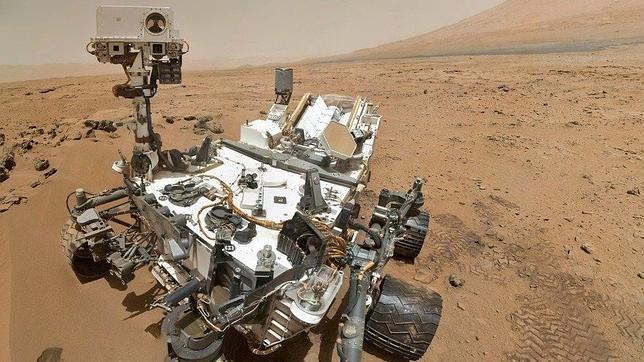
\includegraphics[scale=0.41]{imag/curiosity_marte.jpg}}\hspace{10mm}
	\subfloat[Teleoperación médica]{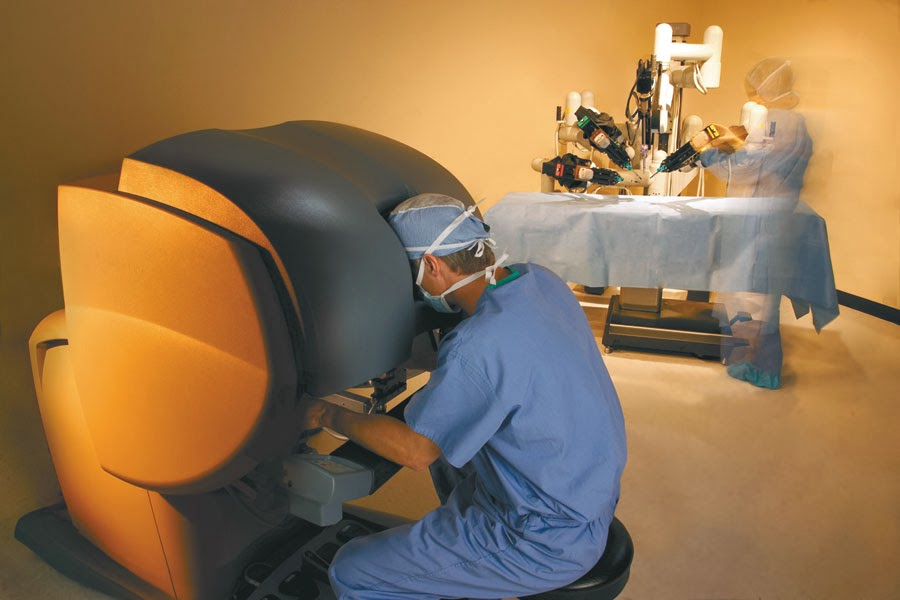
\includegraphics[scale=0.2]{imag/teleoperacion.jpg}}
	\caption{Ejemplos de robots}
	\label{FIG:1_robotica}
\end{figure}

\subsection{Aplicaciones actuales}\label{SEC:Aplic_actual}

Hoy en día, las aplicaciones de los robots son muy diversas. Fuera y dentro de nuestro planeta, los robots permiten ver sitios en los que el hombre no puede llegar directamente o en los que el hábitat es hostil como el Global Explorer ROV, que se ha sumergido en diferentes océanos para obtener imágenes nunca antes vistas por el hombre.

\subsubsection{Sector industrial}

Es uno de los sectores que compra más  robots y se encuentra en constante crecimiento. China pasó en 2013 a los E.E.U.U. en densidad de robots por trabajador y el número de ventas de robots industriales en el mundo aumentó un 16\%  en 2016 por cuarto año consecutivo (Figura \ref{FIG:_robotSales}\footnote{Datos obtenidos de International Federation of Robotics http://www.ifr.org/}\label{FN:IFR}). 

\begin{figure}[hbtp]
	\centering
	\subfloat{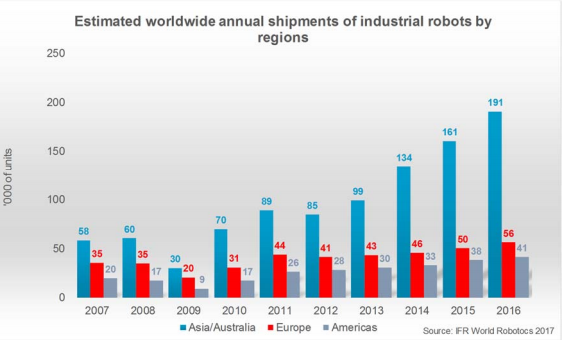
\includegraphics[scale=0.75]{imag/robotSales.png}}
	\caption{Ventas anuales estimadas de robots industriales por regiones}
	\label{FIG:_robotSales}
\end{figure}

Dentro de las aplicaciones industriales de robots encontramos:

\begin{itemize}
	\item Operaciones de manipulación: Usan pinzas, colaboran con otros robots y/u operarios y desplazan objetos. Este uso es uno de los más extendidos en empresas. Por ejemplo en el montaje de coches, ayudando a operarios a desplazar objetos pesados como las puertas.
	\item Soldadores. Se encargan de las tareas de soldadura de componentes. La compañía Asus ha creado un método de producción automático para sus tarjetas gráficas. En concreto, este proceso de soldadura mejora la calidad del producto y permite reducir el tamaño de sus tarjetas notablemente.\footnote{ASUS Auto-Extreme Technology: \url{https://www.youtube.com/watch?v=zVDEcu6-G3s}}
	\item Montaje. Las cadenas de montaje se vuelven más rápidas y eficientes. En las plantas de procesadores Intel, el proceso de montaje es uno de los más avanzados del mundo y se utilizan salas en las que el aire no es respirable para personas y garantizan una densidad de partículas externas muy baja, muy importante para la pureza de los procesadores.
\end{itemize}

\subsubsection{Aplicaciones de servicios}

El acercamiento de los robots a la población ha supuesto que su uso se encuentre en constante crecimiento y el número de aplicaciones es muy variado, desde recreación pasando por la grabación profesional para cine. A continuación se recogen algunas de las aplicaciones ilustrativas:

\begin{itemize}
	\item Limpieza doméstica: Incluye robots que limpian piscinas, hasta aspiradoras inteligentes. Este último caso es el de Roomba, de la compañía iRobot, que incorpora algoritmos de construcción de mapas, evasión de objetos o incluso detección de escaleras (para evitar posibles accidentes).
	
	\item Transporte de personas: Los mayores representante de este tipo de productos son Waymo, Tesla y Uber(Figura \ref{FIG:1_Aplicaciones}). En esta categoría se recogen sistemas de seguridad que controlan la distancia de seguridad respecto de otros vehículos, los sistemas de aparcamiento asistido o habilitar a personas con movilidad reducida o discapacitados para que puedan usar los automóviles. Para ejecutar estas tareas los vehículos están equipados con todo tipo de sensores que permiten la autolocalización, evitar accidentes y llegar al destino deseado. Algunas compañías como Uber y Tesla han sufrido recientemente accidentes mortales que pueden retrasar esta aplicación en el futuro.
	
	\item Ocio y entretenimiento: La utilización de drones con la capacidad de volar ha reducido considerablemente el coste de planos aéreos y simplificado el equipo necesario. Airdog (Figura \ref{FIG:1_Aplicaciones}) es un proyecto nacido de una campaña Kickstarter que permite el seguimiento de actividades deportivas o recreativas a gran velocidad, de forma totalmente autónoma, y la grabación de las mismas.
	
	\item Educación: La aplicación de robots para el uso didáctico se contempla como un recurso innovador, que aumenta el interés de los niños y sirve de apoyo para los maestros (Figura \ref{FIG:1_Aplicaciones}).
	
	\item Militar y seguridad: Para evitar la pérdida de bajas humanas, aumentar la capacidad de motorización y mejorar su potencia de combate. Los ejércitos están invirtiendo cada vez más en robots capaces de sustituir a soldados en el frente y como armas de defensa.
	
\end{itemize}

\begin{figure}[hbtp]
	\centering
	\subfloat[Tecnología Tesla autopilot]{\includegraphics[scale=0.21]{imag/tesla-autopilot.jpg}}\hspace{5mm}
	\subfloat[Secuencia de seguimiento de un Airdog]{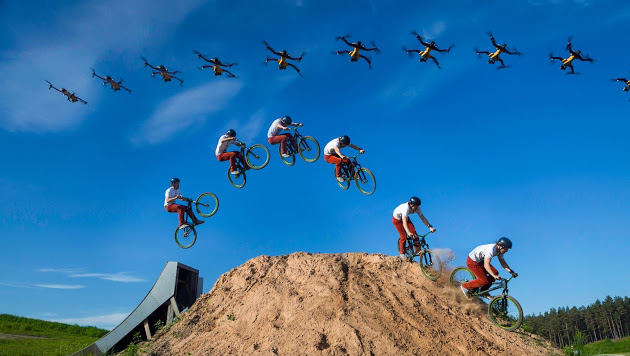
\includegraphics[scale=0.21]{imag/air_dog.jpg}}\hspace{5mm}
	\subfloat[Robot PEPPER en un aula como complemento educador]{\includegraphics[scale=0.4]{imag/pepper.jpeg}}\hspace{5mm}
	\caption{Aplicaciones en la actualidad}
	\label{FIG:1_Aplicaciones}
\end{figure}

\section{Software en robots}\label{SEC:Software en robots}

El software que se encuentra en los robots es el encargado de dotar de un comportamiento inteligente a los mismos. 

Puede estar formado por sistemas complejos, aplicaciones e infraestructuras que son las responsables de las acciones del robot. Las fases del desarrollo del software robótico son muy similares a las del desarrollo de software en otros ámbitos, donde a partir de ciertos requisitos, se modela un diseño que será implementado. Durante años este desarrollo se ha centrado en resolver los problemas con soluciones \textquoteleft ad-hoc\textquoteright, es decir, creando un diseño para un robot con sensores y actuadores específicos. Esto requería que se realizase una implementación nueva por cada robot diferente, a pesar de que las características fueran similares. En la actualidad, gracias a la existencia de diferentes plataformas de desarrollo para robots es posible diseñar e implementar soluciones que puedan aplicarse de forma eficiente y genérica. Esto permite reutilizar herramientas, aplicaciones y algoritmos creados con antelación y reducir los costes durante la fase de desarrollo del software.


\subsection{Simulación}\label{SEC:Simulacion}

Una parte muy importante a la hora de diseñar el comportamiento de un robot es la simulación ya que permite probar algoritmos sin necesidad de utilizar uno real. Esto nos aporta información muy valiosa y facilita la familiarización con posibles situaciones que no hayamos pensado con suficiente antelación, además de prevenir accidentes como por ejemplo cualquier daño físico al robot o herir a las personas cercanas. Una vez se alcance un comportamiento que cumpla nuestras expectativas, se procederá a ponerlo a prueba en el robot real teniendo en cuenta que muy probablemente aparecerán anomalías en el comportamiento no detectadas durante la fase de simulación. Esta diferencia en el comportamiento depende de la precisión con la que se ha caracterizado el modelo del robot y el escenario virtual con el que interacciona. Esto se debe a siempre existe un grado de aproximación entre la virtualización y el mundo real. Muchos simuladores incluyen la adición de funciones de ruido en sensores y actuadores para alcanzar un comportamiento mucho más próximo al real.

Un ejemplo es Gazebo\footnote{Página web oficial de Gazebo : \url{http://gazebosim.org/}}, un proyecto de software libre que incluye multitud de modelos y motores de física virtualizada. Ofrece una interfaz gráfica y control sobre los objetos y el mundo generado, además de la creación y modificación de actuadores y sensores personalizados. Por ejemplo, se pueden crear vehículos con diferentes sensores o casas con las que interactuar.

\begin{figure}[hbtp]
	\centering
	{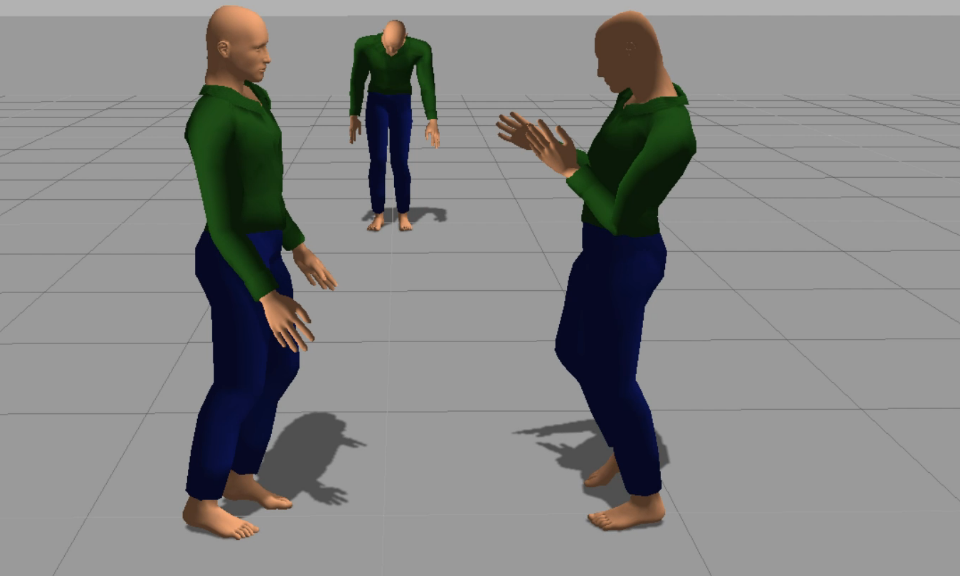
\includegraphics[scale=0.3]{imag/gazebo2.png}}\hspace{10mm}
	%\subfloat[Personas en Gazebo]{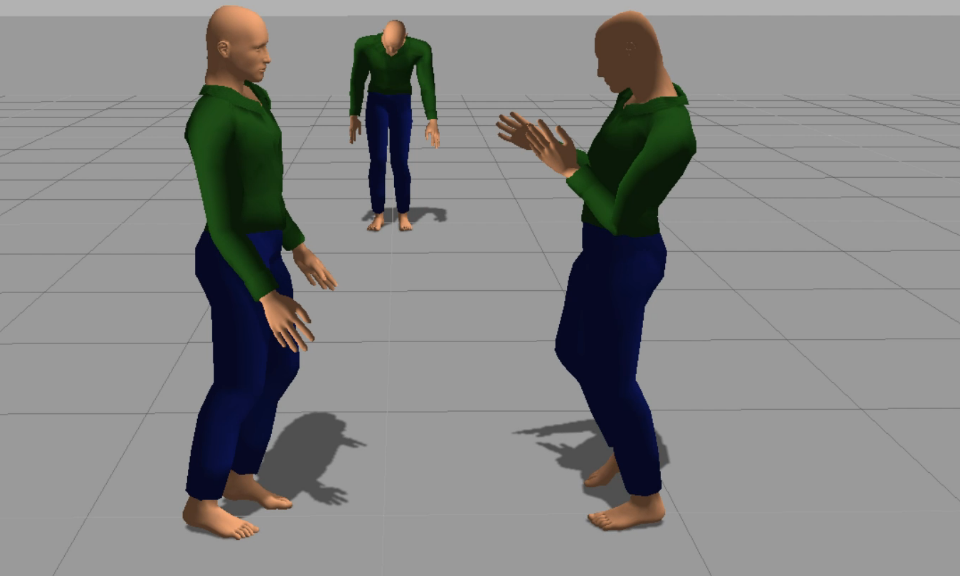
\includegraphics[scale=0.26]{imag/gazebo2.png}}
	\caption{Personas simuladas en Gazebo}
	
	\label{FIG:6_simulacion}
\end{figure}


\section{Visión artificial en robots}\label{SEC:Vision artificial en robots}

La visión artificial, también conocida como visión por computador, es un subcampo de la inteligencia artificial en la que mediante el procesado y análisis de imágenes se trata de extraer información en un computador aplicando transformaciones y algoritmos basados en diferentes disciplinas como por ejemplo la estadística, geometría o \textit{machine learning}.

La visión para los robots, al igual que para las personas, es una gran fuente de información del entorno. Las personas utilizamos el espectro visible de la luz, que se corresponde con lo que llamamos colores. Además, percibimos el mundo que nos rodea como un mundo en tres dimensiones debido a que tenemos dos ojos. Esto nos permite obtener propiedades del entorno y poder  desplazarnos en él sin preocupaciones. Los robots utilizan sensores de visión de todo tipo, capaces de ver en la oscuridad o distinguir diferentes temperaturas. Además, en los últimos años, los sensores de visión han disminuido en precio y su utilización se ha visto incrementada notablemente en el mundo de la robótica, pasando a ser un equipamiento muy común en los robots. En este TFG, utilizaremos dos cámaras para obtener las imágenes que una vez procesadas aportarán la información necesaria para dotar de un comportamiento autónomo al drone.

Existen diferentes bibliotecas que recogen algoritmos y herramientas para simplificar la visión artificial. Cabe destacar \textit{OpenCV}, como la biblioteca  de código libre más extendida a la hora de realizar visión artificial en robots. Esta biblioteca, de la que hablaremos más adelante en detalle \ref{sec:opencvs}, ha facilitado la introducción y la aplicación de técnicas avanzadas de visión artificial para realizar el análisis y procesado de imágenes. Además, podemos encontrar en Internet numerosos ejemplos y tutoriales en los que se muestran las capacidades y aplicaciones de esta biblioteca.

\textit{DeepLearning} (aprendizaje jerárquico), es una familia de técnicas de procesamiento de imágenes basada en \textit{machine learning}. En los últimos años la aplicación de estas técnicas ha dado muy buenos resultados, especialmente dotando de una mayor robustez en comparación a los algoritmos más tradicionales creados para una tarea en específico. 

Actualmente, las aplicaciones de visión artificial en robots son muy variadas, desde seguridad, como sistemas de detección de movimiento, pasando por el entretenimiento, como el sensor Kinect, hasta la accesibilidad para dotar de autonomía a personas que lo necesitan. Para esto se utilizan las siguientes técnicas: 

\begin{itemize}
	\item Construcción de mapas: Es una de las primeras aplicaciones a través de visión y permite a los robots la creación de mapas a través de la detección de bordes, formas o profundidad. Ésta información sirve también para poder navegar sobre sitios desconocidos o previamente han sido convertidos a un mapa \ref{FIG:5_vision}.
	\item Autolocalización: Permite extraer información a un robot sobre la posición relativa respecto al resto del mundo que lo rodea, mediante el reconocimiento de patrones o balizas. Una técnica es el SLAM \ref{FIG:5_vision} (\textit{Simultaneous Localization and Mapping}), que permite la autolocalización al mismo tiempo que se realiza un mapa del entorno. 
	\item Detección e identificación de objetos: El reconocimiento o identificación de objetos\ref{FIG:5_vision} se consigue a partir de la extracción de características únicas de cualquier objeto o persona que podemos encontrar en una imagen. La aplicación de DeepLearning está llevando cada vez más lejos los límites de este reconocimiento, dando lugar a un reconocimiento de objetos mucho más robusto, superando al ser humano en determinadas condiciones.
	\item Navegación y control visual: Permite la navegación autónoma o asistida de robots. Actualmente, se emplea en entornos industriales o el sector de la automoción para el desplazamiento de objetos o personas.
\end{itemize}

\begin{figure}[hbtp]
	\centering
	\subfloat[Reconocimiento de objetos en imagen]{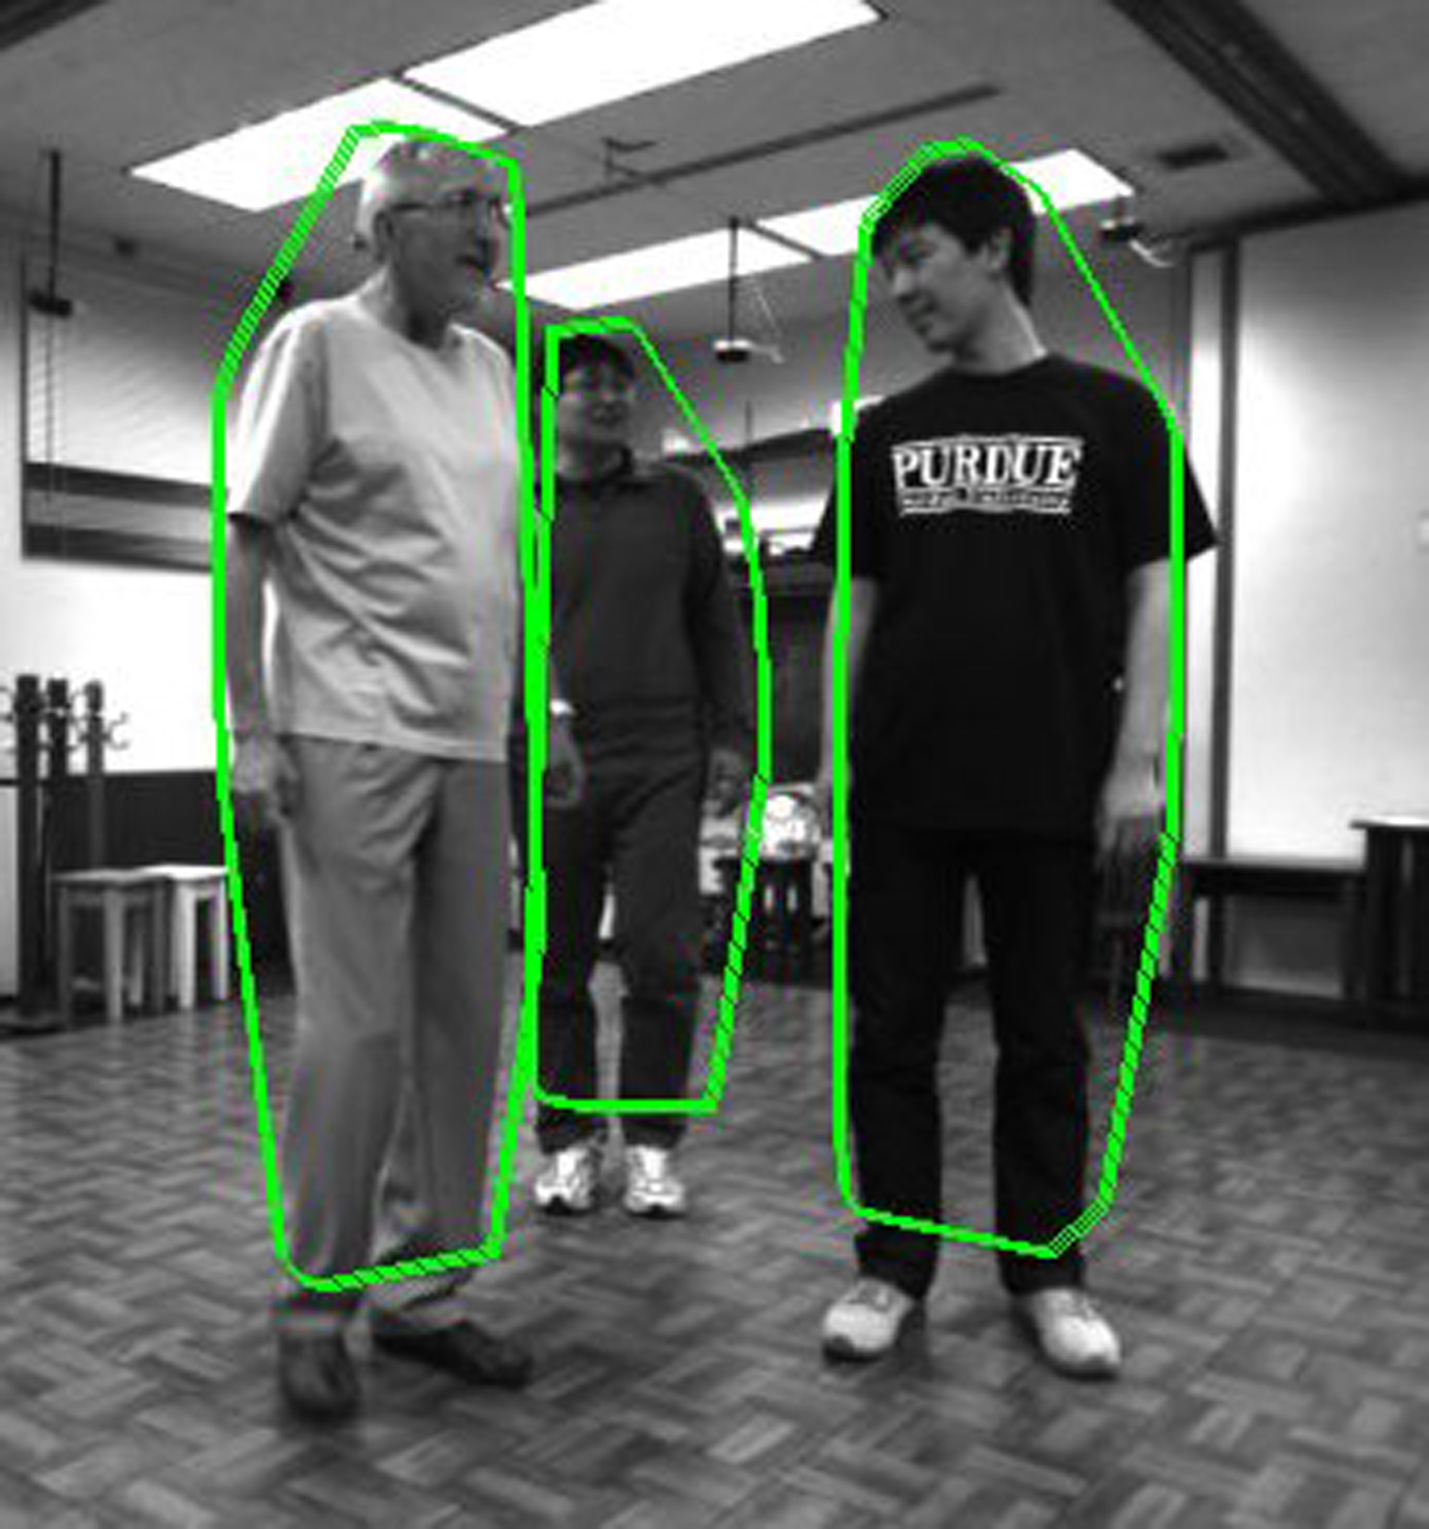
\includegraphics[scale=0.4]{imag/robotic_vision1.jpg}}\hspace{10mm}
	\subfloat[Reconstrucción de mapas con técnicas SLAM]{\includegraphics[scale=0.255]{imag/mapaimagen.jpg}}
	\caption{Visión artificial en robots}
	
	\label{FIG:5_vision}
\end{figure}


\section{Robótica Aérea}\label{SEC:Robotica Aerea}

Es una de las ramas de la robótica de mayor auge actualmente y sus aplicaciones son cada vez más extendidas. Pertenecen a este área los \textit{Unmanned Aircraft Vehicle}(UAV), en español \textit{Vehículo Aéreo No Tripulado}(VANT), o también conocidos como \textit{drones}. Se trata de un vehículo capaz de volar, que puede o no recibir órdenes del exterior. Incluyen multitud de diferentes sensores para mantenerse en vuelo, aterrizar o despegar.

Históricamente, el origen de los UAV ha sido en aplicaciones militares, como en otras áreas de investigación. Una vez ha sido suficientemente desarrollado comienzan las aplicaciones civiles y su aplicación comercial e industrial.
Durante la primera y la segunda guerra mundial se utilizaron drones para la obtención de mapas sin poner en peligro al piloto. Más tarde, en 1995 se utilizaron en Bosnia para tareas de vigilancia o análisis de daños, siendo especialmente importante para el reconocimiento nocturno. El modelo se llamaba \textit{Predator} \ref{FIG:8_historia2}.

\begin{figure}[hbtp]
	\centering
	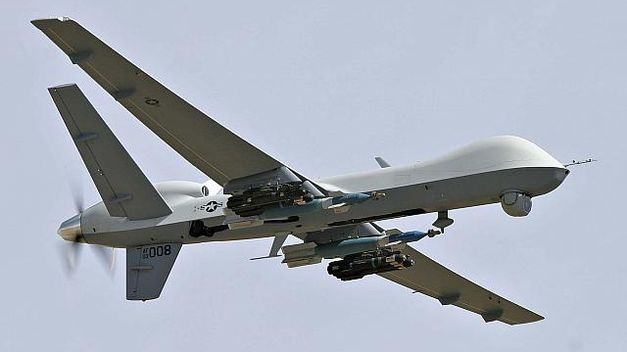
\includegraphics[scale=0.25]{imag/predator.jpg}
	\caption{UAV Predator.}
	
	\label{FIG:8_historia2}
\end{figure}

\subsection{Aplicaciones actuales}

Actualmente, gracias al avance de la estabilización electrónica, los UAV han alcanzado tamaños mucho más reducidos, como el \textit{Hummingbird}\footnote{Más información en: \url{http://www.avinc.com/nano}} o colibrí en español, de \textit{DARPA}. Además son mucho más ágiles y mecánicamente simples. Han aparecido numerosos usos comerciales y civiles, aunque no desaparece el interés militar. Compañías como \textit{Amazon} \ref{FIG:9_historia2}, están trabajando en proyectos para conseguir crear un sistema de envío de compra a domicilio utilizando \textit{drones}, en concreto \textit{cuadricópteros}.
 
Intel está diseñando comportamientos basados en grupos masivos, creando formaciones en el aire y dotando capacidad de pensamiento en grupo a los drones.
 
Otro de los usos es la exploración aérea, que incluye la inspección de embalses, líneas de alta tensión, campos agrícolas y la vigilancia. Este último caso es el de Alemania, que utiliza drones aéreos para evitar el ataque de grafiteros a vagones de tren\footnote{Alemania pone a prueba drones contra los grafitis: \url{http://www.bbc.com/mundo/noticias/2013/05/130528_tecnologia_drones_graffiti_alemania_aa}}.

Uno de los campeonatos más recientes de programación para UAV es el \textit{Mohamed Bin Zayed International Robotics Challenge}(MBZIRC)\footnote{Página Web oficial del campeonato: \url{http://www.mbzirc.com/}}. Con una recompensa de 5 millones de dólares, una de las pruebas consiste en localizar, seguir y aterrizar, coincidiendo con los objetivos principales de este Trabajo Fin de Grado.

\begin{figure}[hbtp]
	\centering
	\subfloat[Modelo utilizado por Amazon Air Prime.]{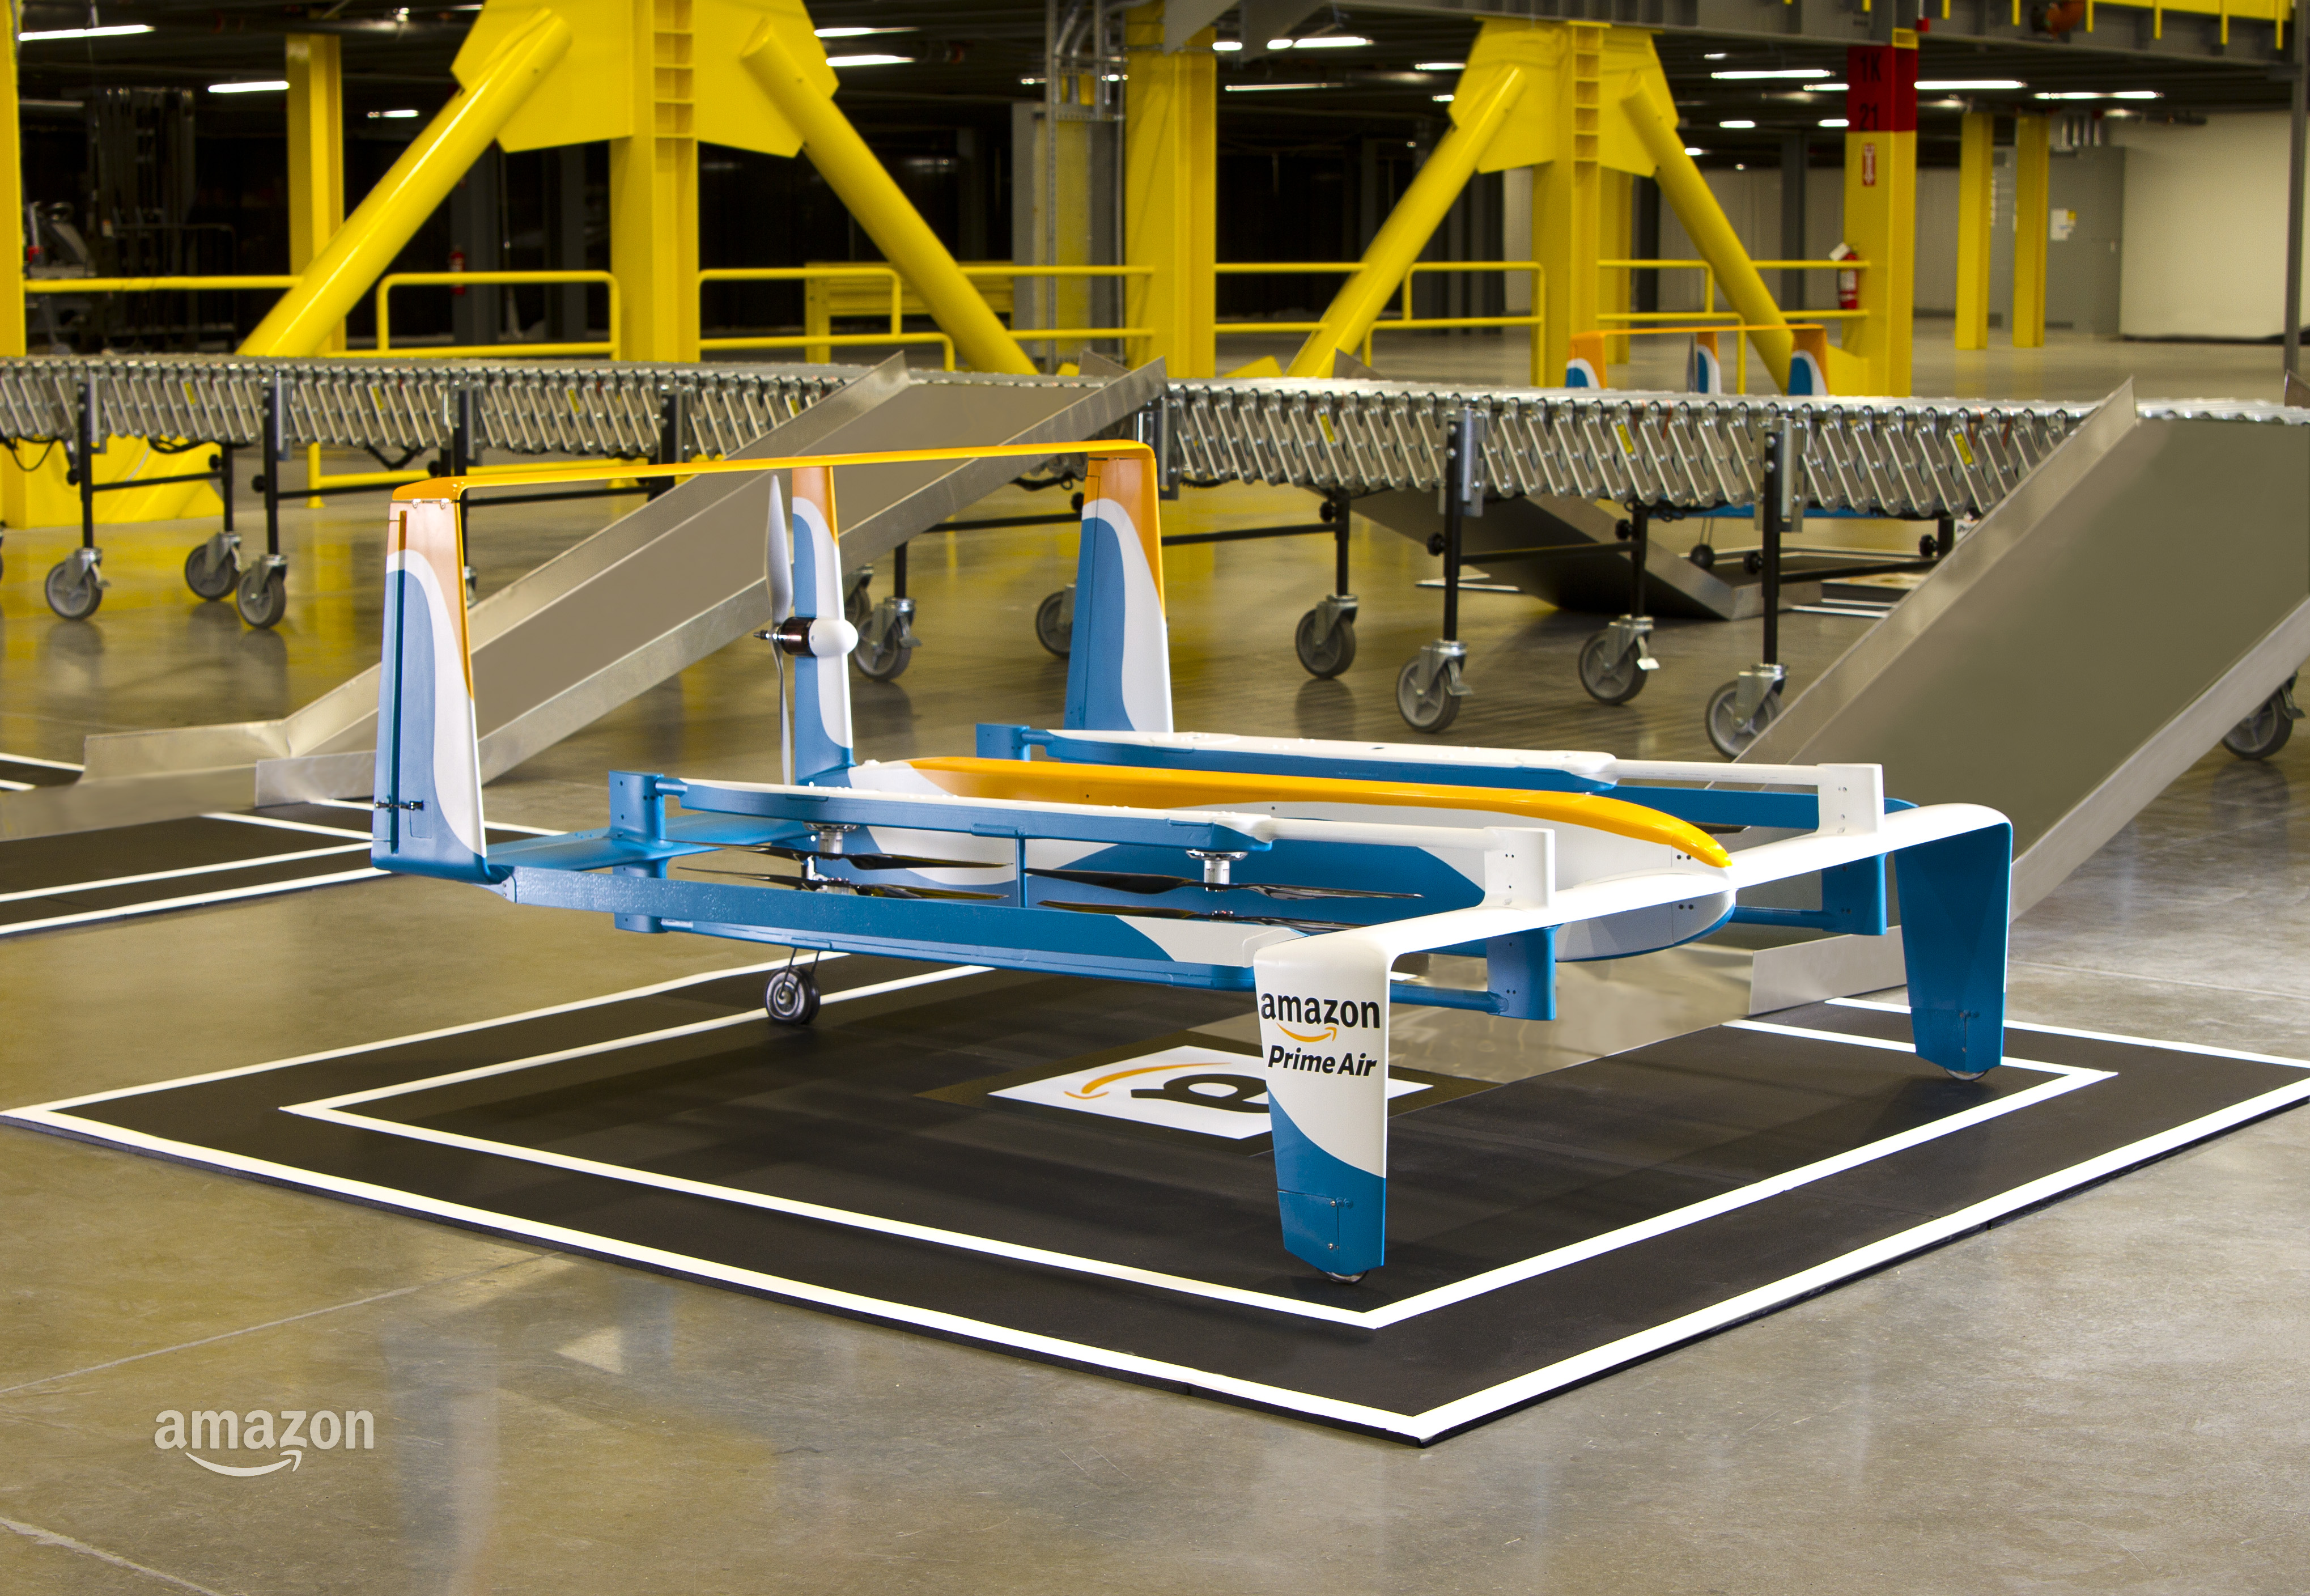
\includegraphics[scale=0.14]{imag/prime-air_03.jpg}}\hspace{5mm}
	\subfloat[Actuación de drones masivos durante la de apertura de los J.J.O.O de Invierno 2018]{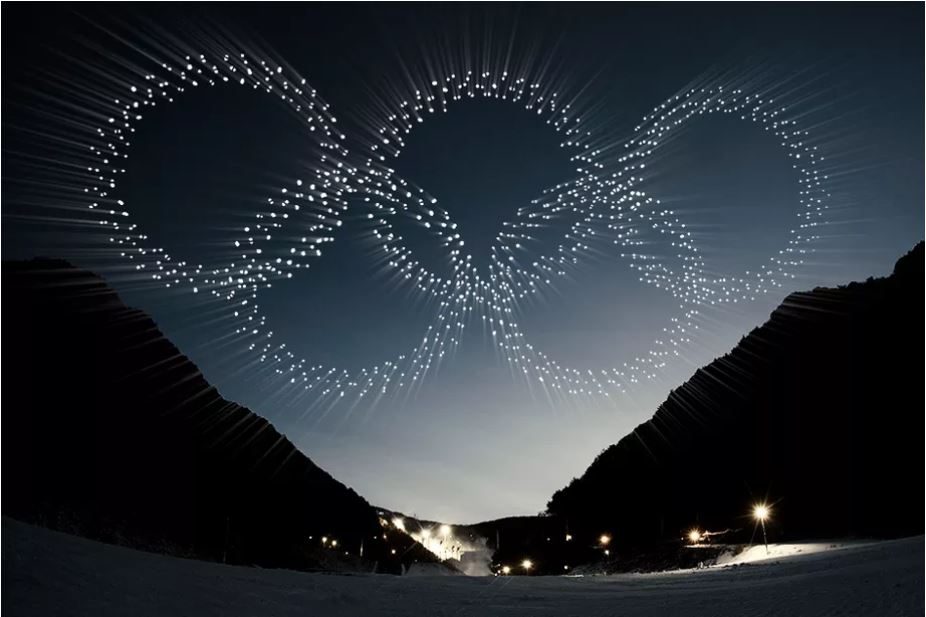
\includegraphics[scale=0.26]{imag/inteldrones.jpg}}
	\caption{Ejemplos de UAV civiles}	
	\label{FIG:9_historia2}
\end{figure}

\subsubsection{Cuadricópteros}

Existen diferentes tipos de drones en función del diseño y los componentes que los forman. Algunos son similares a los aviones, con alas y el mismo método de despegue y aterrizaje. Están pensados para largos períodos de tiempo y altas velocidades. Otros buscan una excepcional maniobrabilidad y estabilidad aérea. En este caso utilizan rotores, al igual que los helicópteros. A este grupo pertenecen los cuadricópteros. Se caracterizan por ser un helicóptero multi-rotor de cuatro brazos en forma de cruz. Los rotores se encuentran en el extremo de cada brazo. 

Cuando los motores giran las hélices situadas en ellos generan un fuerza de empuje vertical llamada \textit{sustentación}. Ésta es perpendicular al movimiento de la hélice y depende de la velocidad a la que gira. La suma de cada fuerza en cada rotor produce una resultante. Los diferentes movimientos que puede describir el cuadricóptero se encuentran recogidos en la Figura\ref{FIG:10_historia2}. El color rojo indica que una potencia mayor ha sido aplicada, mientras que el verde, representa una potencia menor. Para evitar un fenómeno que en los helicópteros produce vueltas sobre sí mismo, la disposición de los motores sigue una forma de cruz, en la que cada par opuesto gira en el mismo sentido. Uno en el sentido de las agujas del reloj y el otro anti-horario.

Para que sea posible el despegue (Figura\ref{FIG:10_historia2},e), esta resultante ha de ser superior al peso del UAV. Si es igual, el drone queda cernido en una altitud fija (\textit{hovering}). Para aterrizar sería necesario una resultante menor que el peso del objeto (Figura\ref{FIG:10_historia2},f).

El giro conocido como \textit{yaw} (Figura\ref{FIG:10_historia2},g y h) o \textit{guiñada}, es el giro del plano horizontal al drone. Para girar a la derecha se transmite más potencia al par de rotores que giran en sentido anti-horario. Si la potencia fuera superior en el otro par opuesto, giraría hacia la izquierda sobre sí mismo.

En el supuesto de que sólo uno de los motores aplicase más potencia que los demás, por ejemplo el delantero, el cuadricóptero se desplazaría hacia atrás, inclinando la parte trasera del vehículo hacia arriba. Esto se correspondería con el movimiento llamado \textit{pitch} (Figura\ref{FIG:10_historia2},a y b) o \textit{cabeceo}.

Por último, si aumentamos la potencia en uno de los motores laterales, por ejemplo la derecha, el vehículo se inclinará y trasladará hacia la izquierda, provocando un movimiento conocido como \textit{roll} (Figura\ref{FIG:10_historia2},c y d) o \textit{alabeo}. 

\begin{figure}[hbtp]
	\centering
	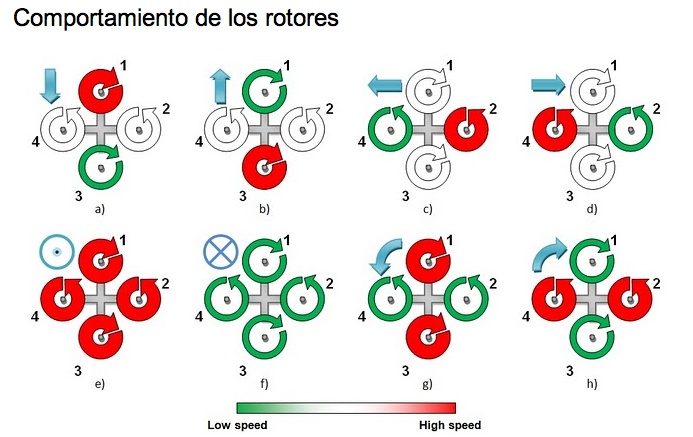
\includegraphics[scale=0.6]{imag/rotores.png}
	\caption{Relación entre la potencia de los rotores y el movimiento de un cuadricóptero}
	\label{FIG:10_historia2}
\end{figure}
Los cuadricópteros pueden tener numerosos sensores a bordo desde acelerómetros, giroscopios, magnetómetros, ultrasonidos, incluso cámaras con resoluciones de hasta 4K. Todo ello se utiliza en combinación para conseguir una mayor estabilización durante el vuelo. Dentro de los actuadores encontramos los cuatro rotores pero también se pueden añadir pinzas para cargar objetos o, en caso de uso militar, armas y sus respectivos gatillos.

Algunos de los fabricantes de cuadricópteros más relevantes actualmente son:

\begin{itemize}
	\item Parrot: Con modelos como el Ar.Drone que acercaron a un gran público el uso de los drones. Actualmente el modelo Bebop 2 \footnote{https://www.parrot.com/us/drones/parrot-bebop-2} ofrece una cámara frontal con resolución \textit{FullHD}, soporte para controles en dispositivos móviles e integración con gafas de realidad virtual para teleoperar el drone.
	\item  Erle: El Erle-Copter \footnote{http://erlerobotics.com/blog/Erle-Copter/} soportado oficialmente por Ubuntu y por el \textit{middleware} robótico ROS (Robot Operating System), facilitando el desarrollo de software en este drone. Está pensado para la instalación de módulos nuevos y así adaptarse a diferentes situaciones.
	\item  DJI: Una de las compañías que más drones vende anualmente, cargados de todo tipo de sensores, cámaras con las últimas tecnologías de estabilización y algoritmos inteligentes de navegación. Su modelo Inspire 2 \footnote{https://www.DJI.com/es/inspire-2?site=brandsite\&from=nav} es muy utilizado en el mundo audiovisual y el cine.
\end{itemize}

\subsubsection{Robótica Aérea en el proyecto JdeRobot}

El proyecto JdeRobot de software libre para robótica lleva años desarrollando proyectos relacionados con la navegación, visión, autolocalización y virtualización de entornos con robots. Gracias a la popularización y a la reducción en coste de los drones se comenzó en el año 2013 una nueva línea de investigación en JdeRobot sobre los UAV. Los primeros proyectos han creado las bases sobre las que seguir investigando y han proporcionado la infraestructura necesaria. Sirven como base antecedentes directos y contexto cercano de este TFG.

Entre estos proyectos se encuentra el Trabajo de Fin de Grado(TFG) \textit{Navegación visual en robots aéreos} de Alberto Martín \cite{AlbertoMartin}. Sus aportaciones fueron la de un driver llamado \textit{ardrone\_server}, que crea una interfaz capaz de comunicarse con el \textit{AR.Drone} de la compañía Parrot. El mismo trabajo incluye una herramienta llamada \textit{uav\_viewer} \ref{FIG:11_uav_viewer}, cuya función es obtener la información de los sensores y teleoperar los actuadores de dicho UAV. Por último, aportó un componente de visión y navegación llamado \textit{object\_tracking} que utiliza filtros de colores para el seguimiento de objetos a través de las imágenes recibidas por la cámara frontal y ventral del drone. El drone es  capaz de un seguimiento autónomo de objetos, tanto en el suelo como en 3D.

\begin{figure}[hbtp]
	\centering
	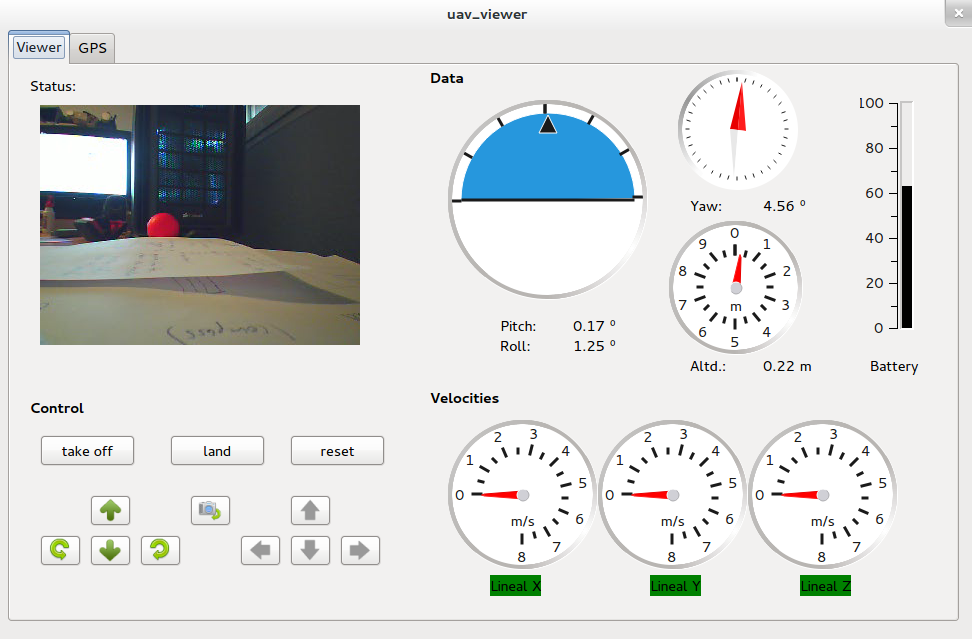
\includegraphics[scale=0.35]{imag/uav_viewer.png}
	\caption{Ejemplo de interfaz de usuario del componentes Uav\_viewer}	
	\label{FIG:11_uav_viewer}
\end{figure}

Daniel Yagüe en su Proyecto Fin de Carrera \textit{Cuadricóptero AR.Drone en Gazebo y JdeRobot} \cite{DanielYague}, desarrolló un modelo y un driver en el simulador Gazebo del mismo AR.drone \ref{FIG:ardronegazebo} que utilizó Alberto Martín. Esto permite tanto la simulación de los datos sensoriales como de la virtualización realista de un comportamiento cercano a dicho drone. Adicionalmente, programó diferentes aplicaciones de navegación autónomas como el seguimiento de balizas por posición, de carretera o de otro cuadricóptero.

\begin{figure}[hbtp]
	\centering
	\subfloat[Modelo de Ar.Drone en Gazebo.]{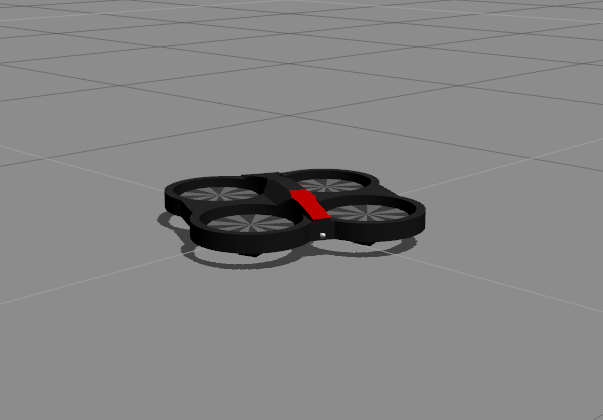
\includegraphics[scale=0.311]{imag/ArDrone_model.png}}\hspace{5mm}
	\subfloat[Modelo Ar.Drone teleoperado en Gazebo]{\includegraphics[scale=0.19]{imag/danielyaguedrone.jpg}}
	\caption{Ejemplos de ArDrone simulado en Gazebo}	
	\label{FIG:ardronegazebo}
\end{figure}

Por otro lado Alberto López-Cerón, con su TFM \textit{Autolocalización visual robusta basada en marcadores} \cite{AlbertoLopez}, creó un algoritmo capaz de estimar la posición de la cámara a partir de la detección de marcadores o balizas. Manuel Zafra siguió desarrollando la idea de Alberto López-Cerón en \textit{Seguimiento de rutas 3D por un drone con autolocalización visual con balizas} \cite{ManuelZafra}. Diseñó un algoritmo de navegación en interiores basado en autolocalización mediante la visión artificial en simulador \ref{FIG:ejemploautolocalizacion}.

\begin{figure}[hbtp]
	\centering
	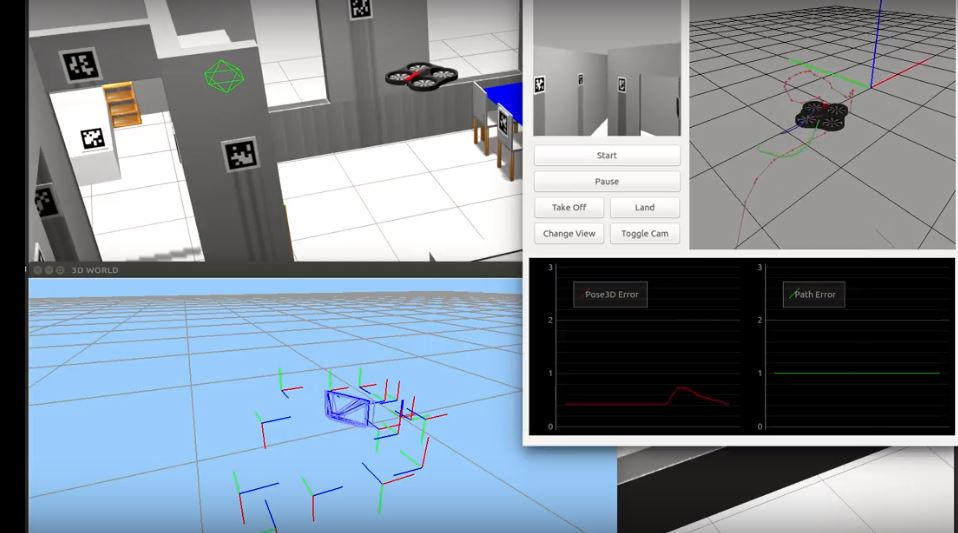
\includegraphics[scale=0.55]{imag/ejemploautolocalizacion.jpg}
	\caption{Ejemplo de algoritmo de navegación basado en autolocalización en Gazebo.}	
	\label{FIG:ejemploautolocalizacion}
\end{figure}


Jorge Vela se centró en el \textit{Despegue, navegación y aterrizaje visuales de un drone usando JdeRobot} \cite{JorgeVela}. Sentó las bases para el despegue y aterrizaje controlado utilizando visión artificial en un drone real \ref{FIG:despgueyaterrizaje}

\begin{figure}[hbtp]
	\centering
	\subfloat[Algoritmo de despegue y aterrizaje encontrando la baliza visual en Gazabo.]{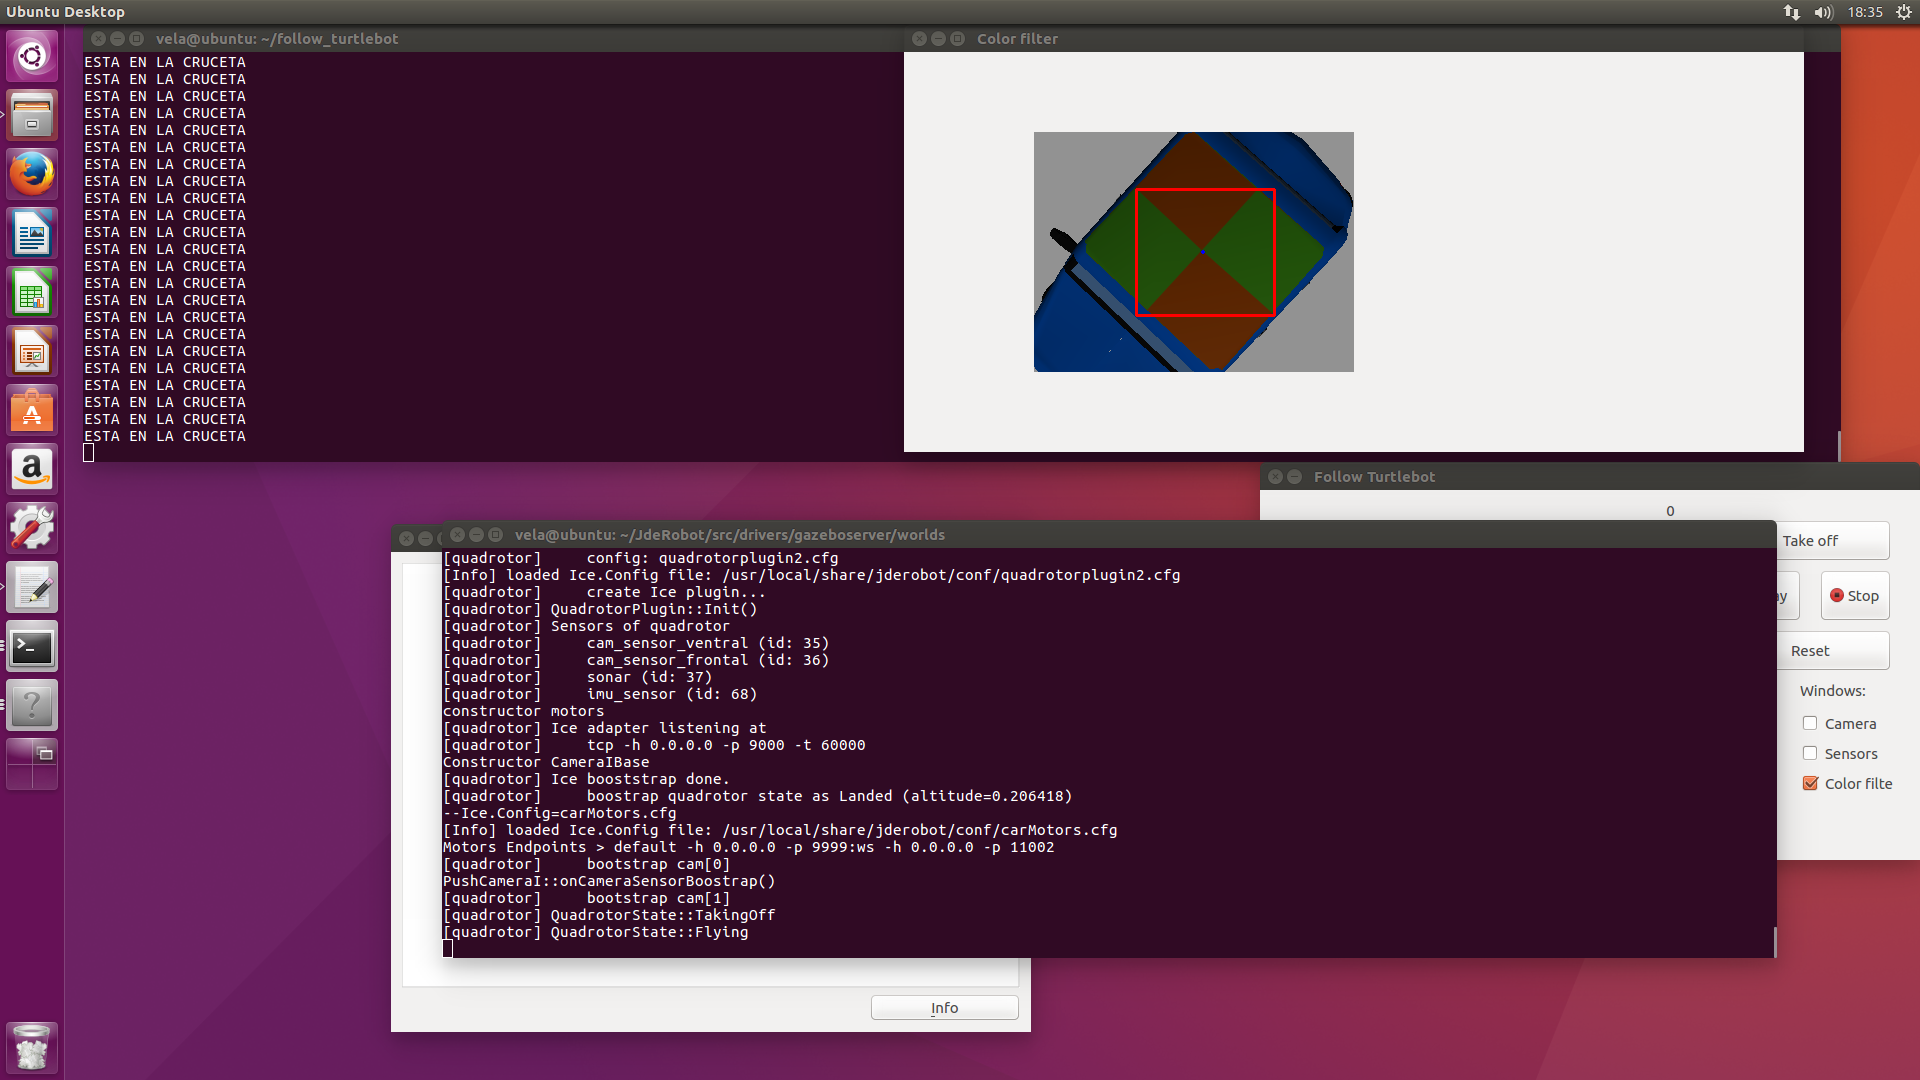
\includegraphics[scale=0.12]{imag/L_CenteringCar.png}}\hspace{2mm}
	\subfloat[Ar.Drone en vuelo sobre baliza visual.]{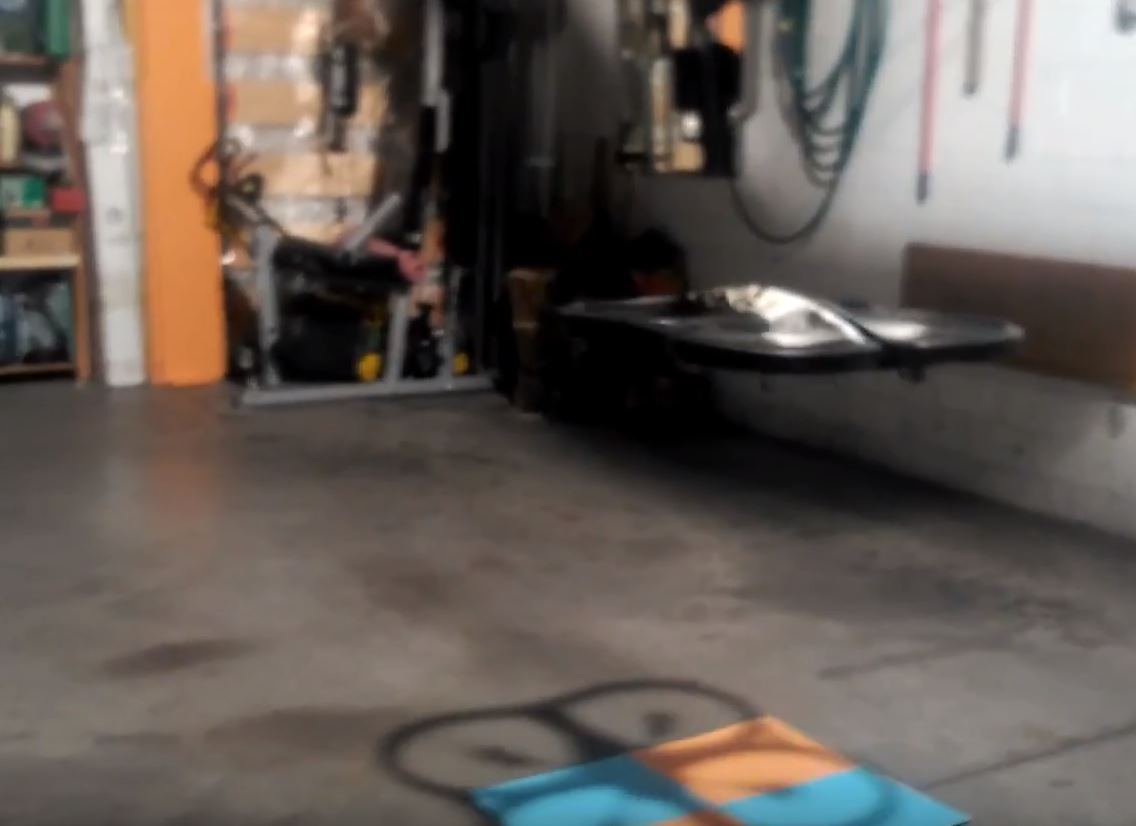
\includegraphics[scale=0.22]{imag/aterrizajereal.jpg}}
	\caption{Ejemplos de aterrizaje y despegue en Gazebo y el drone real.}	
	\label{FIG:despgueyaterrizaje}
\end{figure}

Jesús Saiz, en su TFG \textit{Programación de un drone para seguimiento autónomo de trayectorias en 3D} \cite{JesusSaiz}, integró el algoritmo de despegue y aterrizaje controlados y la autolocalización visual basada en balizas para crear un autómata de estados finito que navega de forma autónoma a través de rutas predefinidas en el simulador Gazebo. 

\begin{figure}[hbtp]
	\centering
	\includegraphics[scale=0.25]{imag/SlamMarkersJesus.jpg}
	\caption{Ejemplo de navegación a través del seguimiento de rutas.}	
	\label{FIG:ejemplonavegacion}
\end{figure}



Siguiendo con las bases aportadas por todos estos proyectos, en este TFG se programará el comportamiento autónomo de despegue controlado y aterrizaje de un drone sobre una baliza visual y la navegación a partir de la autolocalización. Se utilizará un drone real, empleando la infraestructura existente en JdeRobot para estos cuadricópteros. Con ello se pretende unificar los avances anteriores en un drone real y dejó la puerta abierta a nuevos comportamientos más sofisticados.


En el próximo capítulo se explicarán los objetivos y la metodología propuesta para resolverlos. En el tercer capítulo se expondrán con profundidad la infraestructura y herramientas  utilizadas. En el cuarto, se describirá el desarrollo de todos los componentes que forman este proyecto. En quinto lugar, se detallarán los distintos experimentos para validar experimentalmente la solución programada. Para terminar, unas conclusiones aportarán un visión global del conjunto y los conocimientos extraídos.


%\lhead[]{CAPÍTULO \thechapter. OBJETIVOS}
\chapter{Objetivos}\label{cap.objetivos}
En este capítulo describiremos los objetivos planteados para el Trabajo de Fin de Grado, los requisitos exigidos y la metodología utilizada para el desarrollo.

\section{Problema a abordar}
\label{sec:objetivos}

El objetivo principal de este trabajo es desarrollar una aplicación que a través de técnicas de visión artificial dote de navegación autónoma a un drone real. El resultado consistirá en un despegue, una navegación en tres dimensiones guiada por balizas y por último, una fase de aterrizaje.

Este objetivo global se ha dividido en varios subobjetivos concretos:

\begin{itemize}
	
	\item \textbf{Desarrollo e integración del módulo de autolocalización 3D a partir de balizas visuales:} Este módulo proporciona la posición relativa del drone basándose en la detección de balizas visuales y cálculos geométricos. Dentro del proyecto JdeRobot existe un módulo basado en los trabajos previos mencionados en el capítulo anterior \cite{AlbertoLopez} \cite{ManuelZafra} \cite{JesusSaiz} que será revisado, refinado e integrado en la aplicación final.
	
	\item \textbf{Desarrollo e integración de un módulo de navegación por balizas visuales:} Este módulo será el encargado de buscar y navegar en un entorno real utilizando información del módulo de autolocalización basado en balizas visuales. La navegación deberá ser totalmente autónoma (sin teleoperación).
	
	%\item \textbf{Desarrollo de una aplicación para la calibración de balizas bicolor arlequinadas:} Esta aplicación es fundamental para acelerar el proceso de calibración y de operaciones morfológicas necesarias, a través de una interfaz de usuario sencilla. Generará un fichero de configuración fácilmente transferible que será utilizado por los módulos de despegue y aterrizaje.
	
	%\item \textbf{Implementación e integración de módulos de búsqueda:} Se desarrollarán dos módulos de búsqueda. El primero estará basado en la búsqueda en espiral del TFG de Jorge, siendo necesaria su integración con la aplicación final. El segundo tipo de búsqueda es de tipo rotacional y está utilizará el módulo de autolocalización. El dron girará sobre sí mismo hasta que encuentre la baliza visual que tiene como objetivo.
	
	\item \textbf{Programación del comportamiento del drone  en un autómata de estados finito:} La aplicación final será un único algoritmo basado en un autómata de estados finito que tendrá las siguientes fases: Despegue, aterrizaje, búsqueda y navegación basada en balizas visuales. Esta programación se apoyará en el despegue y aterrizaje existentes en el proyecto de JdeRobot \cite{JorgeVela} \cite{JesusSaiz}, que se refinarán y adaptarán utilizando la herramienta de autómatas \texttt{VisualStates}.
	
	\item \textbf{Validación experimental en el cuadricóptero  real} Se realizarán pruebas unitarias para validar los diferentes módulos constituyentes y pruebas del sistema completo para demostrar el correcto funcionamiento de la solución desarrollada. Se explorarán varias configuraciones ejecutando el software tanto en un ordenador externo como en un ordenador a bordo del cuadricóptero.
	
\end{itemize}

\section{Requisitos}
\label{sec:requisitos}

La solución desarrollada deberá satisfacer, adicionalmente, los siguientes requisitos:

\begin{itemize}
	
	\item Los componentes y aplicaciones desarrollados han de estar integrados en la plataforma JdeRobot-5.6.4.
	
	\item El control de navegación del cuadricóptero ha de ser fluido y ágil, de modo que pueda mantenerse estable al menos 5 segundos en cada baliza, evitando en todo momento perder del campo de visión el objetivo.
	
	\item Los componentes y aplicaciones desarrollados han de ser computacionalmente eficientes y deben ser modulares.
	
	\item El sistema operativo debe estar basado en la distribución GNU/Linux Ubuntu 16.04.
	
	\item Programado en el lenguaje Python, versión 2.7.
	
\end{itemize}

\section{Metodología}

Para materializar los objetivos y requisitos previamente mencionados es necesario aplicar algún método que defina las distintas etapas y estados. En este Trabajo de Fin de Grado se aplica el método de desarrollo en espiral. Este modelo, creado por Barry Boehm en 1986, se utiliza frecuentemente en la ingeniería de software. Se basa en una serie de iteraciones en bucle. En cada ciclo, se realiza un conjunto de cuatro actividades:

\begin{enumerate}
	\item \textbf{Determinar los objetivos}: Poner limitaciones definidas en forma de objetivos o requisitos. Dividir el proyecto en partes más pequeñas.
	\item \textbf{Análisis del riesgo}: Estudiar los riesgos de cada uno de los objetivos que se abordan. Evaluar las alternativas posibles en caso de amenazas.
	\item \textbf{Desarrollar y probar}: Verificación de la tarea actual. Al mismo tiempo, se realiza un análisis para encontrar nuevos factores de riesgo, como errores que se podrían arrastran a la próxima iteración.
	\item \textbf{Planificación}: Establecer y definir las fases anteriores.
\end{enumerate}

\begin{figure}[h]
	\centering
	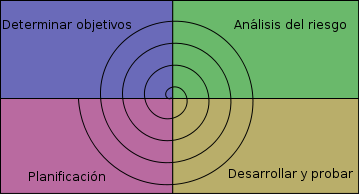
\includegraphics[width=90mm]{imag/desarrollo_en_espiral.png}
	\caption{Representación del desarrollo en espiral.}
	\label{fig:21_planificacion_espiral}
\end{figure}

Durante el desarrollo de este proyecto se han establecido reuniones periódicas con el tutor. En ellas revisábamos los objetivos anteriormente fijados y los resultados obtenidos. Si alguno de los objetivos generaba algún problema o no se llegaba al resultado deseado, se aplazaban o se profundizaba en la raíz del problema. A continuación se determinaban los objetivos de nuestro próximo encuentro. 

Como parte de la evaluación de los objetivos propuestos, ha sido fundamental la utilización del mediawiki\footnote{http://JdeRobot.org/Andresjhe-tfg}  de la plataforma JdeRobot. En él están publicados, a modo de cuaderno de bitácora, los hitos y progresos, incluyendo también imágenes o vídeos. 

Para el seguimiento y almacenamiento del software desarrollado se ha empleado la herramienta de control de versiones GIT. Todo el código relacionado con este proyecto es software libre y es accesible en el repositorio\footnote{https://github.com/RoboticsURJC-students/2014-tfg-Andres-Hernandez}.

\section{Planificación}

Para conseguir los objetivos fijados anteriormente se ha seguido el siguiente plan de trabajo:

\begin{itemize}
	
	\item \textbf{Formación y familiarización con el entorno JdeRobot:} Incluye el preparación de las dependencias necesarias para la instalación del entorno. Estudio de las diferentes bibliotecas, interfaces y componentes. Aprendizaje y profundización de lenguajes de programación como Python y C++, así como la herramienta para las comunicaciones ICE y la biblioteca de visión OpenCV.
	
	\item \textbf{Aprendizaje de la herramienta VisualStates:} Necesaria para la generación de autómatas de estado finito. Se han generado varios ejemplos para conocer las diferentes secciones, para la inserción de variables, funciones y nuevos estados.
	
	\item \textbf{Aprendizaje e implementación del módulo de despegue, búsqueda en espiral y aterrizaje:} Necesario para conocer el funcionamiento del los antecedentes ya existentes de control de un drone para seguir una ruta de control de un drone para aterrizar usando visión. Se ha adaptado y mejorado el código para ganar rendimiento y robusted. También se han buscado soluciones propias de control y se han integrado todos en una máquina de estados finito programada con la herramienta \texttt{VisualStates}.
	
	\item \textbf{Aprendizaje y familiarización con técnicas de autolocalización desde balizas visuales:} Necesario para conocer el funcionamiento de las balizas visuales y cómo obtener las diferentes coordenadas a partir de su detección. Se ha realizado el estudio de antecedentes existentes en el proyecto JdeRobot \cite{AlbertoLopez} \cite{ManuelZafra} junto a la información publicada en la página oficial de AprilTags \footnote{https://april.eecs.umich.edu/}. 
	
	\item \textbf{Validación experimental:} Se ha diseñado una secuencia de pruebas unitarias para poder validar incrementalmente la solución, siendo la última prueba un ejercicio que reunirá y ejecutará de principio a fin las pruebas unitarias anteriormente realizadas y validadas. Ha sido necesaria la instalación de sistema operativo, herramientas y aplicaciones en el co-procesador para poder ejecutar la aplicación final.
	
\end{itemize}

%\lhead[]{CAPÍTULO \thechapter. INFRAESTRUCTURA}
\chapter{Infraestructura}\label{cap.infraestructura}
En este capítulo se describen los programas y dispositivos en los que nos hemos apoyado para la elaboración de este proyecto.
Debido a la naturaleza de la plataforma JdeRobot, el sistema operativo que se ha elegido para el desarrollo y ejecución de los componentes ha sido Linux (la distribución Ubuntu 16.04) y el lenguaje de programación Python (versión 2.7 para compatibilidad de JdeRobot con ROS-Kinetic).

\section{Parrot Ar.Drone 2}

Este es el drone que ha utilizado durante las pruebas reales. Parrot\footnote{https://www.parrot.com/global/} es un fabricante de dispositivos de diferente naturaleza, que van desde manos libres para teléfonos pasando por todo tipo de robots. Fue uno de los fabricantes que más popularizaron los drones a partir de 2010 con su primer Ar.Drone.

Este drone está dotado de una API de comunicaciones que forma parte de un SDK\footnote{http://developer.parrot.com/} que proporciona el fabricante de manera gratuita para obtener los datos de los sensores y/o control de los motores del cuadricóptero. Se ha utilizado la versión 2.4.

Posee dos cámaras, una ventral y otra frontal, incluye un acelerómetro y todo el procesado se realiza en un ARM de dos núcleos a bordo. Por último, está dotado de Wi-Fi como canal de comunicaciones por defecto y genera un punto de acceso sin contraseña para que los dispositivos se conecten y comuniquen con él. 

%%%%%%
%%%%%%\section{Interfaz Gráfica de usuario}
%%%%%%También conocida como \textit{GUI}, es el software encargado de simplificar la interacción con los usuarios. Proporciona texto, imágenes y diferentes objetos gráficos para representar la información y e interactuar con las acciones que se ofrezcan en un programa.

%%%%%%\subsection{Qt}
%%%%%%Qt\footnote{http://www.qt.io/} es una biblioteca multiplataforma cuyo objetivo principal es el de facilitar el diseño de interfaces gráficas de usuario. Su modelo de desarrollo es el de software libre y de Código Abierto, bajo la licencia GPL v3 y LGPL v2.1. Está programada en C++ , aunque puede ser utilizada junto a otros lenguajes de programación, como por ejemplo PyQt en Python. Ofrece un \textit{ambiente de desarrollo integrado}(IDE en inglés) llamado QtCreator, que facilita el proceso de desarrollo y el diseño gráfico del GUI. La versión utilizada en este proyecto es la 4.8.

%%%%%%\begin{figure}[H]
%%%%%%\centering
{%%%%%%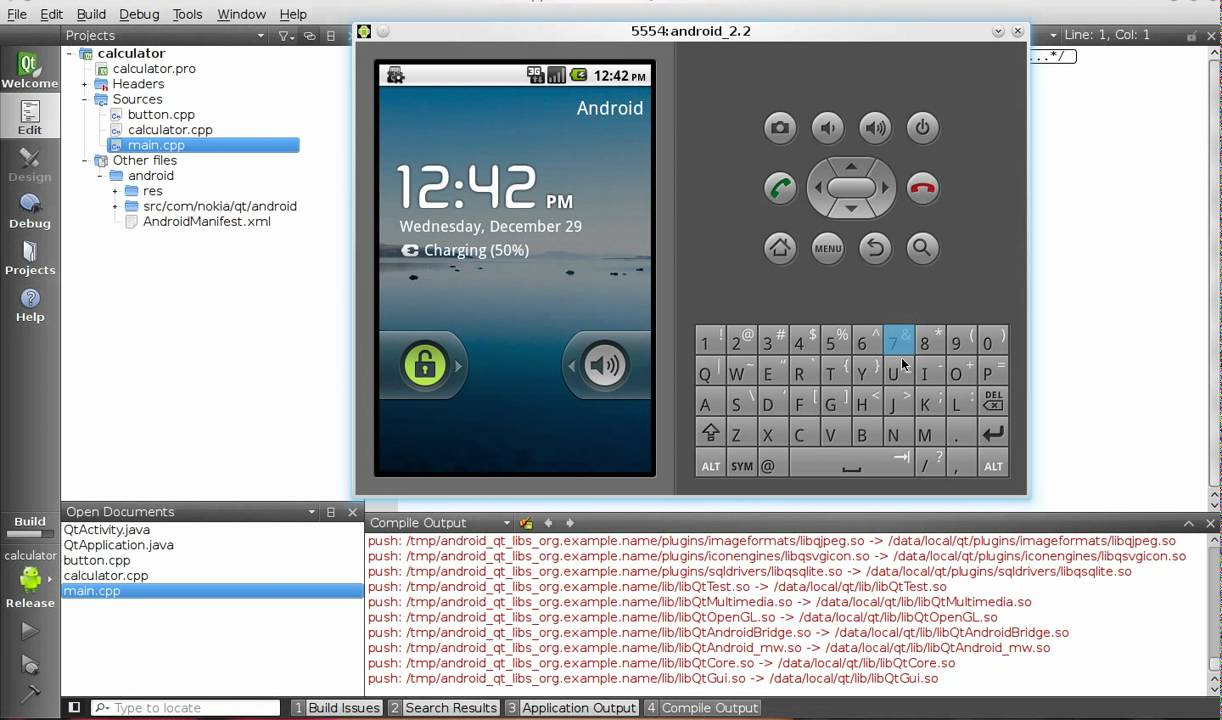
\includegraphics[scale=0.2]{imag/qt.jpg}}\hspace{10mm}
	%\subfloat[Personas en Gazebo]{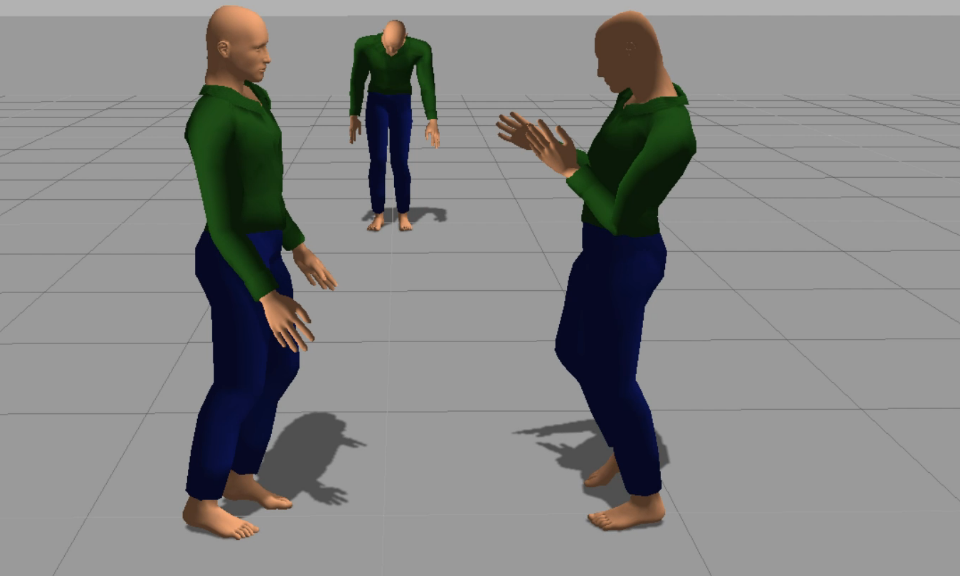
\includegraphics[scale=0.26]{imag/gazebo2.png}}
	%%%%%%\caption{Qt Creator}
	
	%%%%%%\label{FIG:31_qtcreator}
	%%%%%%\end{figure}
	
	%%%%%%\subsubsection{PyQt}
	
	%%%%%%PyQt\footnote{https://riverbankcomputing.com/software/pyqt/intro} es una colección de bibliotecas escritas en Python y C++ que complementan Qt. Mantiene la característica multiplataforma  y es un partner reconocido oficialmente por el propio Qt. Se encuentra bajo la licencia GPL v3 y la \textit{Riverbank Commercial License}. En este proyecto se ha utilizado para el desarrollo de componentes utilizando el lenguaje de programación Python. La versión utilizada en este proyecto es la PyQt5.
	
	\section{Intel Compute Stick}
	\label{sec:ics}
	
	Para dotar de autonomía y potencia de procesado al Ar.Drone 2, se ha decidido utilizar un co-procesador a bordo. Se ha utilizado este dispositivo Intel Compute Stick que entra dentro de la categoría de \textit{miniordenadores} u ordenadores de tamaño reducido. La principal ventaja es su relación peso y rendimiento, ya que está equipado con un procesador de dos núcleos, capaz de ejecutar 4 hilos simultáneamente. Cuenta con Wi-Fi integrado, además de un puerto USB, lector de tarjetas SD y HDMI como salido de vídeo.
	
	\begin{figure}[H]
		\centering
		\includegraphics[scale=0.6]{imag/ics.jpg}
		\caption{Imagen de Intel compute Stick}
		\label{FIG:34_ics}
	\end{figure}
	
	\section{Biblioteca OpenCV} \label{sec:opencvs}
	
	OpenCV\footnote{https://opencv.org/} es una biblioteca de visión artificial de código abierto, que tiene un conjunto de transformaciones y operaciones con imágenes o matrices que facilitan el procesamiento de las mismas. Es el estándar internacional de facto en procesamiento de imágenes. Está programada en C++ y Python y en este TFG se ha utilizado la versión 3.4.
	
	En este proyecto se ha utilizado para realizar filtros de color en imágenes para identificar la balizas de despegue y aterrizaje. Otro uso es para realizar transformaciones morfológicas en imágenes como la erosión y la dilatación, que permiten eliminar la sombra que proyecto el drone. Por último, de esta biblioteca también se han utilizado transformaciones geométricas de matrices para estimar la posición relativas del drone a partir de la información de balizas en una imagen de dos dimensiones.
	
	\section{Biblioteca AprilTags}
	\label{sec:AprilTags}
	
	En este proyecto se utilizará una librería de balizas visuales denominada \textit{AprilTags} \footnote{https://april.eecs.umich.edu/software/apriltag/}. Es un sistema de visualización fiduciaria. Estas balizas se basan es símbolos diseñados para ser fácilmente reconocidos del resto del entorno \ref{FIG:33_apriltag}. Puede detectar uno o varios símbolos en la misma imagen, además de proporcionar información como la identificación y posición de cada símbolo dentro de una imagen de cada uno. Es un sistema robusto cuyo funcionamiento es independiente del ángulo y diferentes situaciones de luminosidad en la imagen.
	
	\begin{figure}[H]
		\centering
		{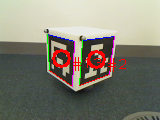
\includegraphics[scale=1.56]{imag/apriltag.png}}
		%\subfloat[Personas en Gazebo]{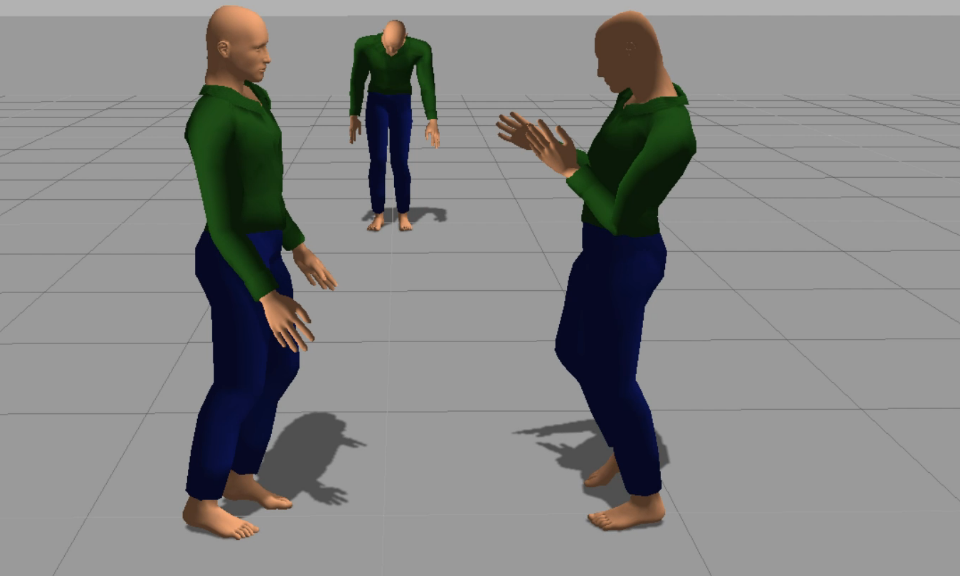
\includegraphics[scale=0.26]{imag/gazebo2.png}}
		\caption{Ejemplo de detección en AprilTag}
		
		\label{FIG:33_apriltag}
	\end{figure}
	
	
	Los símbolos se dividen en diferentes familias. Estas familias utilizan un número de bits y de distancia de Hamming predefinidos. Dentro de cada familia, se generan los diferentes símbolos, asignando un único ID o identificador. Esto permite el reconocimiento en caso de tener varias balizas al mismo tiempo en el campo de visión.
	
	Sus aplicaciones son muy variadas, desde la captura de movimiento en objetos hasta sistemas de navegación basada en balizas. Otra de sus aplicaciones es la de realidad aumentada, sustituyendo el símbolo por una imagen virtualizada.
	
	Además del sistema de balizas se proporciona una biblioteca que ofrece funciones de identificación de estas balizas en imágenes. Esta biblioteca está escrita en C y Java pero Ed Olson de Massachusetts Institute of Technology (MIT) ha creado una adaptación en C++. El código\footnote{https://svn.csail.mit.edu/apriltags} es abierto y está protegido bajo la LGPL v2.1. Entre sus dependencias se encuentran OpenCV y Eigen3, ambas son bibliotecas de tratamiento de imagen en Linux. A través de la utilización de un recubrimiento \footnote{https://github.com/swatbotics/AprilTag/toree/máster/Python} para Python ha sido posible su integración con la aplicación final de este TFG.
	
	\begin{figure}[H]
		\centering
		{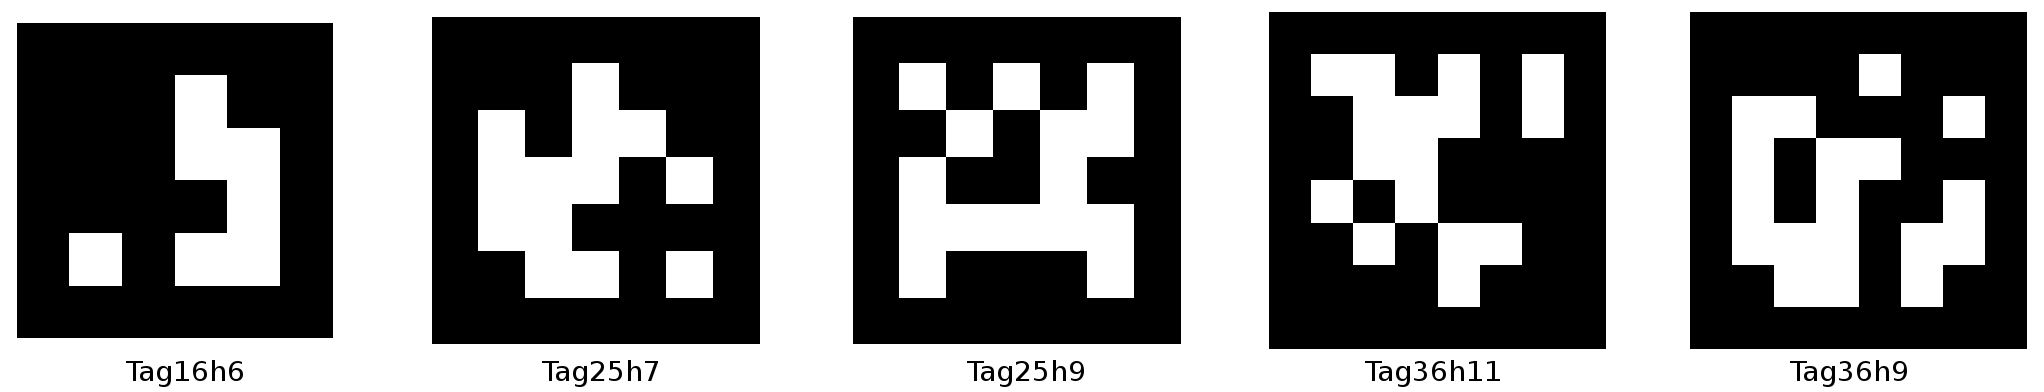
\includegraphics[scale=0.2]{imag/apriltags-codes.png}}
		%\subfloat[Personas en Gazebo]{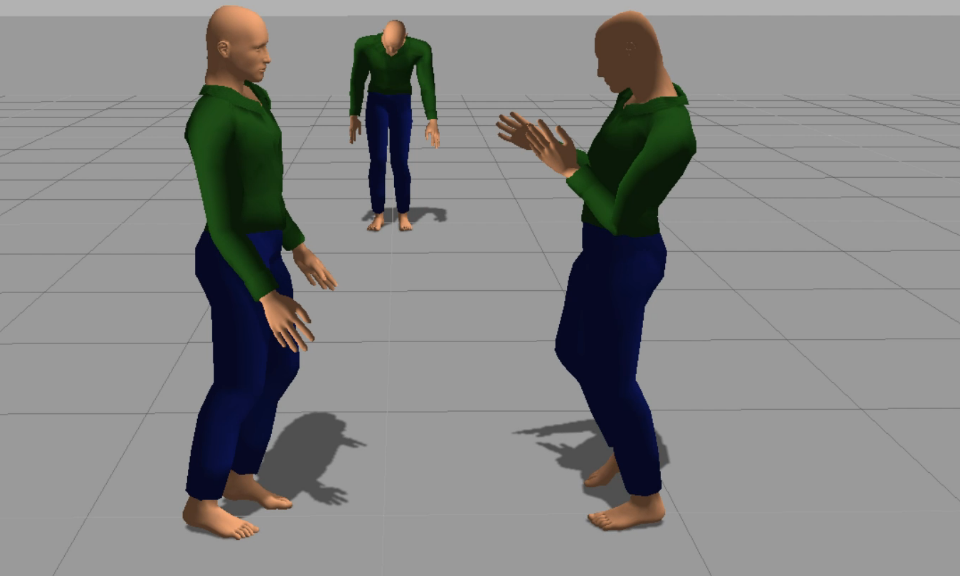
\includegraphics[scale=0.26]{imag/gazebo2.png}}
		\caption{Ejemplos de familias en AprilTag}
		
		\label{FIG:34_apriltag_families}
	\end{figure}
	
	
	\section{Entorno JdeRobot}
	\label{sec:Jderobot}
	
	En el mundo de la robótica existen diferentes plataformas que simplifican y aportan las herramientas necesario para el desarrollo de aplicaciones en robots. JdeRobot es una de ellas y consiste en una colección de drivers, herramientas y bibliotecas robóticas, domóticas y de visión artificial. Estas piezas de software están escritas en diferentes lenguajes como C++ o Python y su interoperación se realiza a través de interfaces ICE o interfaces ROS. En ella participan desarrolladores de diferentes niveles desde profesionales del sector, profesores, alumnos de la Universidad Rey Juan Carlos y de otras universidades internacionales. El código fuente es libre y está bajo la licencia GPL v3 y la documentación se encuentra protegido bajo la licencia de Creative Commons by-SA. La versión utilizada en este proyecto es la 5.6.4\footnote{https://github.com/JdeRobot}.
	
	Durante el desarrollo de este TFG, componentes de esta plataforma como \texttt{uav\_viewer}, \texttt{uav\_viewer\_py}, \texttt{slam\_markers} y \texttt{ardrone\_server} han servido de referencia y han tenido una gran relevancia para el aprendizaje de la plataforma.
	
	Se repasan a continuación los más relacionados con este trabajo:
	
	\subsection{Ardrone\_Server}
	
	Este componente fue desarrollado en el TFG de Alberto  Martín \cite{AlbertoMartin} y permite a partir de un protocolo basado en interfaces ICE el envío y lectura de comandos específicos del SDK del Ar.Drone 2.
	Como resultado, podemos modificar la velocidad de los motores para cambiar la posición del drone, recibir las imágenes de sus cámaras, envío de órdenes predeterminadas como el aterrizaje o despegue, recibir la información de sensores, etcétera.
	
	\begin{figure}[H]
		\centering
		{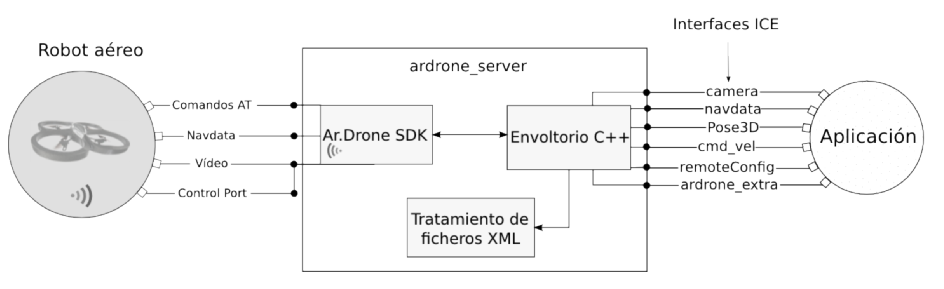
\includegraphics[scale=0.4]{imag/ardrone_server_structure.png}}
		\caption{Estructura de ardrone\_server}
		
		\label{FIG:32_ardrone_server}
	\end{figure}
	
	Está programado en C++ y es absolutamente necesario para cualquier comunicación con el drone real.
	
	
	
	\subsection{Teleoperadores uav\_viewer y uav\_viewer\_py} \label{subsec:uavviewer}
	
	Ambos son componentes de JdeRobot y ofrecen una GUI para enviar comandos tanto al cuadricóptero real, como al Ardrone simulado o mostrar la información de los sensores y cámaras. 
	Los comandos se envían a través de interfaces ICE al componente \texttt{ardrone\_server}, que los transforma a su vez en comandos para el SDK del Ar.Drone 2. La principal diferencia entre ambos es el lenguaje en el que han sido desarrollados: \texttt{uav\_viewer\_py  }está escrito en Python y ofrece un GUI más parecido a los mandos físicos de teleoperación de drones mientras que \texttt{uav\_viewer} \ref{FIG:11_uav_viewer} está en C++.
	
	\subsection{Herramienta Color Tuner}
	\label{subsec:colorTuner}
	Este componente facilita la configuración de filtros de color utilizando OpenCV. En su interfaz gráfica se selecciona el espacio de color que queremos utilizar, RGB, YUV y HSV, siendo esta última la utilizada por nuestras aplicaciones. Dentro de la aplicación, las ventanas \textit{Source image} y \textit{Filtered image} mostrarán la imagen recibida y su versión filtrada respectivamente. Para especificar los valores que se aplicarán para filtrar, se modifica la posición deslizadores o \textit{sliders} que representan los valores máximos y mínimos de H (\textit{hue} o tinte), S (saturación) y V (value o luminosidad).
	
	
	\begin{figure}[H]
		\centering
		{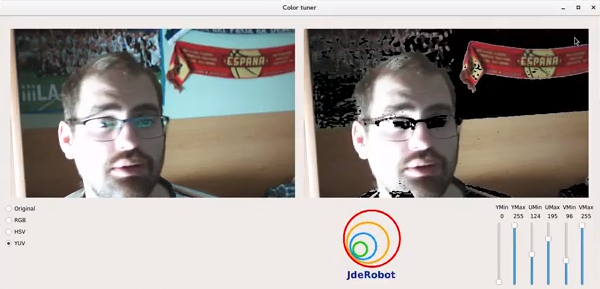
\includegraphics[scale=0.55]{imag/colortuner.png}}
		\caption{Ejemplo de Color Tuner aplicando filtros de color}
		
		\label{FIG:32_colorTuner}
	\end{figure}
	
	
	\subsection{Componente slam\_markers}
	\label{subsec:slam Markers}
	
	Esta herramienta permite mediante la aplicación de una serie de algoritmos de autolocalización basado en balizas visuales. Su algoritmo analiza las imágenes en 2D recibidas por la cámara y utiliza tanto la biblioteca OpenCV como AprilTags. Primero identifica si existen balizas \ref{FIG:32_slamMarkers} Una vez localizada, aplica funciones para calcular la posición y orientación en tres dimensiones de la cámara con respecto a la baliza. En el siguiente paso se ejecuta un proceso de fusión temporal y fusión espacial de la estimación obtenida. Por último, devuelve a través de una interfaz ICE las coordenadas 3D obtenidas como resultado de todo el proceso.
	 
	Ha sido desarrollada por Felipe Pérez en su TFM\footnote{http://jderobot.org/Flperez-tfm}. Ha sido programada en C++ y actualmente se encuentra aún en desarrollo. Para nuestro TFG se ha reimplementado su algoritmo en Python para facilitar la integración con la aplicación final y mejorar el rendimiento.
	
	\begin{figure}[H]
		\centering
		{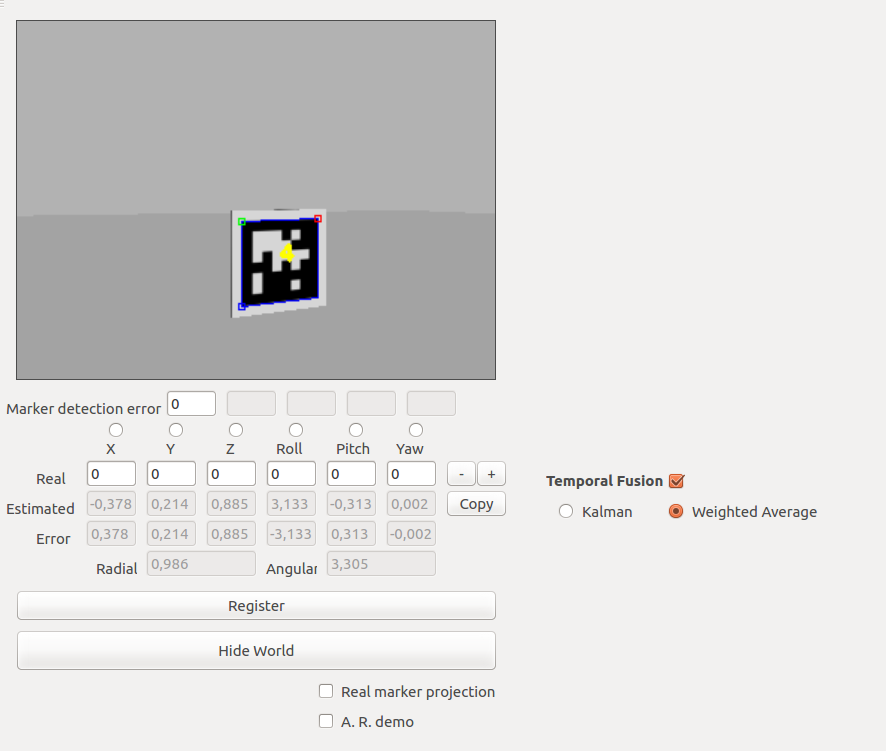
\includegraphics[scale=0.4]{imag/slam_markers_ui.png}}
		\caption{Ejemplo de slam\_markers identificando una baliza}
		
		\label{FIG:32_slamMarkers}
	\end{figure}
	
	
	\subsection{VisualStates}
	\label{subsec:VisualStates}
	
	Esta herramienta\footnote{http://jderobot.org/VisualStates} forma parte de la infraestructura JdeRobot  y su principal función es facilitar la creación de programas para robots basados en máquinas de estados finito con estados y transiciones. 
	
	Se caracteriza por tener una interfaz de usuario en la que podemos generar o modificar estados, teniendo siempre uno como principal a partir del cual comenzará la ejecución.
	Cada estado se compone por un código que será ejecutado en bucle hasta que se realice una transición a otro estado diferente. La herramienta genera como salida un programa que materializa el autómata, y que puede estar escrito tanto en Python como en C++.
	
	Las transiciones se dibujan entre los diferentes estados existentes especificando las condiciones temporales o basadas en variables que provocarán el cambio de estado.
	
	Adicionalmente proporciona un menú de configuración de interfaces ICE compatibles con JdeRobot, una sección de variables y funciones para que se compartan entre los diferentes estados. El menú también permite la modificación de la duración de las iteraciones periódicas en las que se van ejecutando los estados.
	
	Por último, tiene la capacidad de generar ejecutables y sus respectivos ficheros de configuración ICE. Esto facilita el empaquetado y el despliegue de los programas en un único fichero ejecutable.
	
	\begin{figure}[H]
		\centering
		{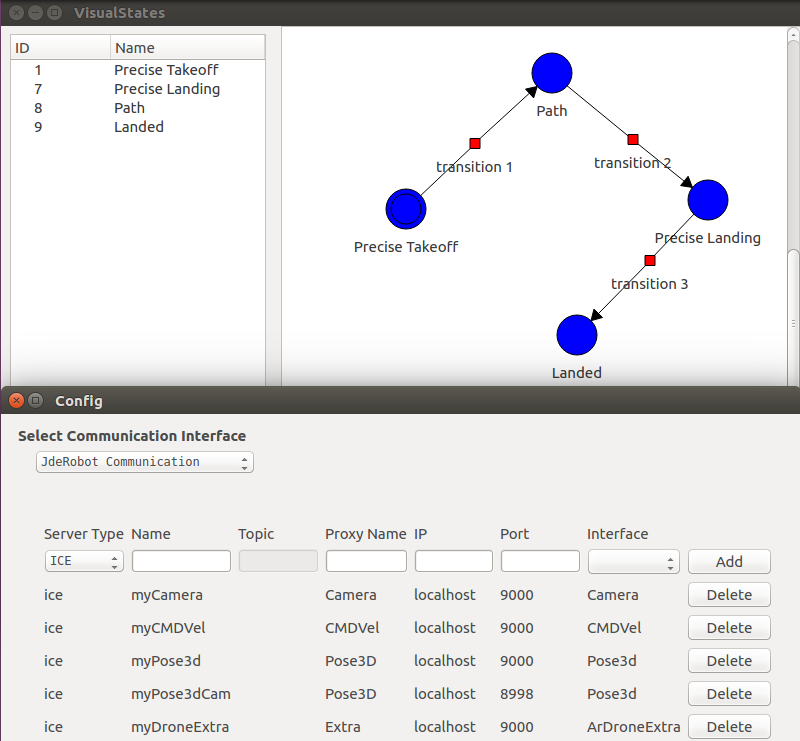
\includegraphics[scale=0.45]{imag/IMG32.png}}
		%\subfloat[Personas en Gazebo]{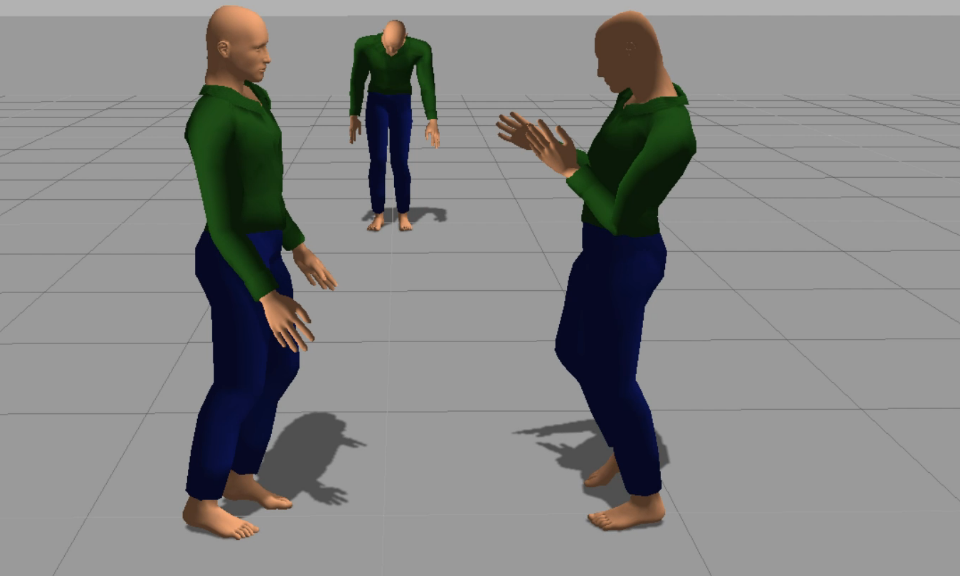
\includegraphics[scale=0.26]{imag/gazebo2.png}}
		\caption{Ejemplo de autómata generado con VisualStates}
		
		\label{FIG:33_visualstates}
	\end{figure} 
	
	\section{Bibliotecas ICE}
	
	ICE\footnote{https://zeroc.com/} es un \textit{middleware} de Código Abierto orientado a objetos que proporciona las herramientas, APIs y librerías necesarias para simplificar las comunicaciones entre componentes usando modelos basados en cliente y servidor y objectos distribuidos. En JdeRobot es la plataforma elegida como infraestructura para las comunicaciones entre nodos. Proporciona una capa transparente que se encarga de abrir y cerrar conexiones, la serialización de información, retransmisión de paquetes perdidos, etcétera. La versión utilizada en este proyecto es la 3.6
	
	\section{Simulador Gazebo}
	
	Este simulador de código abierto es la herramienta en la que se realizarán algunas las pruebas experimentales. En este TFG se ha utilizado la versión Gazebo 7.12 para simular al drone en diferentes escenarios. De este modo podremos evaluar previamente el código antes de ejecutarlo en el drone real. 
	Los escenarios simulados o mundos se crean con la propia aplicación y se definen con la extensión \textquotedblleft\texttt{.world}\textquotedblleft. Están escritos mediante SDF (\textit{Simulation Description Format}) que a su vez, está basado en el lenguaje XML y es muy popular en entornos de simuladores para robots.
	Estos mundos contienen modelos virtuales de robots que pueden tener un papel activo como un drone o pasivo como las balizas. El comportamiento activo se materializa mediante plugins que permiten la ejecución de código, interacciones con el motor de físicas del simulador, la obtención de imágenes desde cámaras virtuales, etcétera.
	
	\begin{figure}[H]
		\centering
		{\includegraphics[scale=0.3]{imag/gazebo-jackal-race.png}}
		\caption{Ejemplo de simulador Gazebo}
		\label{FIG:33_gazebo}
	\end{figure}
	
	%\section{OpenSSH} \label{sec:openssh}
	%Es una herramienta de código abierto para el acceso remoto a través de una autenticación utilizando el protocolo SSH \footnote{https://www.openssh.com/}. El tráfico se envía de forma cifrada para evitar que terceros puedan intervenir o escuchar el intercambio de información. Dispone de una variedad de opciones, métodos de autenticación y la capacidad de abrir túneles punto a punto de forma segura. En este TFG se ha utilizado su versión 7.7 y se ha empleado para intercambiar información entre el co-procesador y el ordenador desde el que queramos iniciar la aplicación final.
%\lhead[]{CAPÍTULO \thechapter. ALGORITMO}
\chapter{Navegación autónoma de un drone guiado por balizas visuales}\label{cap.desarrollo}
En este capítulo se describe la solución desarrollada para conseguir que un drone navegue autónomamente guiado por balizas visuales y utilizando la infraestructura mencionada anteriormente. Se explicará el diseño alto nivel de la solución y se describirá con mayor detalle las partes desarrolladas.

%\hspace{1cm} Para explicar todo los pasos primero se dara un vistazo al diseño globalmente para posteriormente explicar cada uno de los modulos indicidualmete y así poder conocer todos ellos en detalle.

\section{Diseño}
El objetivo de este proyecto es desarrollar un algoritmo para dotar a un drone de un comportamiento completamente autónomo desde el despegue, hasta el aterrizaje, ambos controlados, pasando por la localización y aproximación a diferentes posiciones 3D asociadas a las balizas, pero desconocidas de antemano. Todo esto basándose únicamente en balizas de apoyo visual. 

El componente desarrollado necesita dos ficheros de configuración. Primero un fichero xml llamado \textit{calibration.xml} que almacena los parámetros necesarios para la detección robusta de balizas arlequinadas. Segundo un fichero con la secuencia deseada de balizas AprilTags a las que se quiere que el drone visite en su navegación autónoma.

En la figura \ref{fig:Solucion final} se pueden ver las entradas y salidas de flujos de información. Adicionalmente, se han sido incluido los ficheros  imprescindibles en cada módulo para su correcto funcionamiento. Esto nos dará una imagen de alto nivel de la solución. Las comunicaciones entre procesos se llevan a cabo mediante interfaces de la biblioteca ICE. 

\begin{figure}[H]
	\begin{center}	
	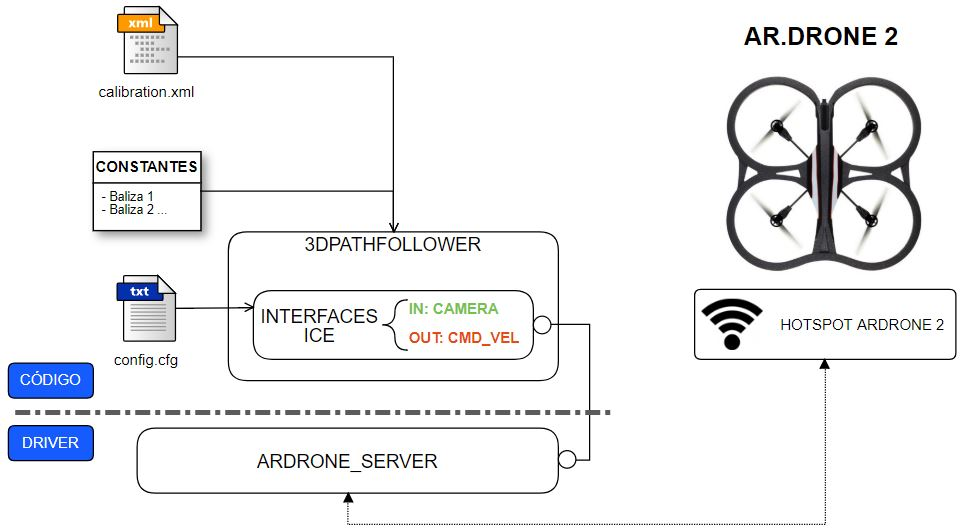
\includegraphics[scale=0.6]{imag/desgin_escenario.jpg}
	\caption{Entradas y salidas de la solución final.}
	\label{fig:Solucion final}
	\end{center}
\end{figure}

El componente 3DPahtFollower es la  aplicación mencionada anteriormente. Está compuesta por los diferentes estados del autómata, tal y como se puede apreciar en la figura \ref{fig:Solucion 3DPathFollower}. Se han agrupado los diferentes estados para una mejor comprensión del despegue controlado, navegación y búsqueda rotacional y por último, búsqueda en espiral y aterrizaje controlado. Cada uno de los estados se componen de una capa de percepción visual, que llevará a cabo la tarea de identificar las balizas y otra capa de control, que calculará y generará el comportamiento que se enviará al drone a través de las interfaces ICE. La navegación autónoma del drone se entiende aquí como la visita en secuencia a una serie de balizas AprilTags que están situadas en posiciones desconocidas por el drone, pero cercanas cada una a la siguiente en la secuencia.

\begin{figure}[H]
	\begin{center}	
		\includegraphics[scale=0.6]{imag/design_pathfollower.png}
		\caption{Diagrama de bloques del componente 3DPathFollower.}
		\label{fig:Solucion 3DPathFollower}
	\end{center}
\end{figure}

A continuación vamos a explicar cada estado y sus respectivas transiciones de las que se compone \textit{3DPathFollower} con mayor profundidad, siendo la creación de un algoritmo de navegación, el diseño de la infraestructura y la aplicación \textit{CalibrationTool} las mayores aportación de este TFG, por lo que serán los apartados en los que haremos mas hincapié. Sin embargo, al tratarse de un TFG de integración también explicaremos los módulos en los que nos hemos basado y los cambios que hemos aplicado para su correcto funcionamiento en el la aplicación final.

\section{Detección visual de las balizas}

La percepción se ha basado en la detección de dos tipos de balizas visuales: Una baliza bicolor para las fases de despegue y aterrizaje y otro tipo de balizas tipo AprilTags. 

\subsection{Balizas de aterrizaje y despegue}

Durante la realización de este TFG ha sido necesaria la configuración de filtros los de color de las balizas en los que se basa principalmente el despegue y aterrizaje controlado de la aplicación principal. Se utiliza la biblioteca de OpenCV para realizar las operaciones sobre imágenes.

Se ha escogido utilizar una baliza de color arlequinada \ref{fig:baliza arlequinada} compuesta por cuatro cuadrantes y 2 colores lo más distantes posibles en el espacio de color HSV (como por ejemplo naranja y verde), colocados de forma no contigua. Esto permitirá aumentar la robustez y reducir los posibles errores que se produzcan debido al ruido de otros colores en el ambiente.

\begin{figure}[H]
	\begin{center}	
		
\includegraphics[scale=0.2]{imag/color_beacon_3.png}
		\caption{Ejemplo de baliza de color arlequinada.}
		\label{fig:baliza arlequinada}
	\end{center}
\end{figure}

\textit{3DPathFollower} utiliza la suma de dos filtros de color, llamados \textit{Primary} y \textit{Secondary} los diferentes valores máximos y mínimos de los componentes HSV y de las transformaciones morfológicas sobre las imágenes filtradas que explicaremos a continuación. Estas transformaciones  son la erosión y dilatación. La combinación de estas técnicas permite la eliminación de impurezas y el suavizado de la imagen, dotando de mayor robustez al filtro de color.

Se aplicará el procesado para cada uno de los dos colores, llamando a la función hsvFilter (importada de Color Tuner) y acto seguido se realizarán las transformaciones morfológicas a la imagen filtrada en HSV:

\begin{lstlisting}[backgroundcolor=\color{gray!15}]
Pmask, PmaskHSV = hsvFilter(PH_max,PS_max,PV_max,
PH_min,PS_min,PV_min,image,hsv)
PmaskHSV = cv2.erode(PmaskHSV,kernel,iterations = PErode)
PmaskHSV = cv2.dilate(PmaskHSV,kernel,iterations = PDilate)
\end{lstlisting}

Donde \textit{kernel} es el tamaño de píxeles al que se aplicará y \textit{iterations} se corresponde con la intensidad.
El resultado consistirá en la suma de ambas imágenes filtradas:
\begin{lstlisting}[backgroundcolor=\color{gray!15}]
filterImage = PmaskHSV+SmaskHSV
\end{lstlisting}

\subsection{Balizas de autolocalización}

Para la identificación de las balizas, tanto durante la búsqueda como la aproximación, se utilizarán las funciones nativas de AprilTags. Necesitaremos crear un detector para nuestra familia (36H11 \ref{FIG:34_apriltag_families}), para más adelante aplicarlo sobre una imagen convertida a escala de grises:

\begin{lstlisting}[backgroundcolor=\color{gray!15}]
self.options = apriltag.DetectorOptions()
self.detector = apriltag.Detector(self.options)
detections = self.interfaces.detector.detect(gray)
\end{lstlisting}

Para obtener esta estimación hemos tomado como referencia el algoritmo utilizado por la aplicación Slam\_Markers \ref{subsec:slam Markers} y lo hemos implementado en el lenguaje Python.

El algoritmo para estimar la posición relativa en 3D a partir de una imagen en 2D, serie de transformaciones y cálculo de matrices que a partir de las cuatro esquinas detectadas por AprilTags obtiene el vector basado en las coordenadas X,Y,Z:

\begin{lstlisting}[backgroundcolor=\color{gray!15}]
retVal,rvec,tvec =cv2.solvePnP(self.interfaces.m_MarkerPoints
,detection.corners
,self.interfaces.cameraMatrix
,self.interfaces.distCoeffs)
rodri = cv2.Rodrigues(rvec)
#We get X,Y and Z
cameraPosition = -np.matrix(rodri[0]).T * np.matrix(tvec) 
self.interfaces.x = cameraPosition.item(0)
self.interfaces.y = cameraPosition.item(1)
self.interfaces.z = cameraPosition.item(2)
\end{lstlisting}

Para calcular conocer la rotación relativa de nuestro drone con respecto a la posición baliza, se realiza una serie de transformaciones que se basan en los ángulos de euler:

\begin{lstlisting}[backgroundcolor=\color{gray!15}]
#We get roll, pitch and yaw from Euler Angles        
eulerAngles = 
self.interfaces.rotationMatrixToEulerAngles(rodri[0])
\end{lstlisting}

\section{Autómata de navegación} 
\label{sec:3Dpathfollow}
Este componente está formado por un algoritmo de navegación autónoma basado en un control representado por un autómata de estados finito. Ha sido realizado con la herramienta \textsc{Visual States}, la cuál nos ha permitido tanto desarrollar el código, como la integración con las diferentes bibliotecas y partes del sistema en un solo programa.

\begin{figure}[H]
	\begin{center}
		\includegraphics[width=0.85\textwidth]{imag/EstadosVisualStates.png}
		\caption{Estados de la aplicación 3DPathFollower}
		\label{fig: EstadosVisualStates.}	
	\end{center}
\end{figure}

En la figura \ref{fig: EstadosVisualStates.} se observan los diferentes estados y transiciones que forman la aplicación. El primer estado es el de \textit{Take-off}, en el que se envía un comando al drone para iniciar los motores en modo despegue para ganar altura y despegarse del suelo. Dado que esta fase tiene una duración de unos 2 segundos, el siguiente estado es el de \textit{Initializatión} en el que, junto a otras tareas de inicialización, se realiza la lectura del archivo de configuración \textit{calibration.xml} mostrado en la Figura \ref{fig:Solucion 3DPathFollower}, del que obtendremos los parámetros para el filtro de color. \textit{Color Beacon Tracking} se encargará de mantener estable y de forma contralada al drone encima de la baliza de color. Transcurridos 4 segundos en el objetivo, damos por estable el despegue y procedemos al estado \textit{AprilTag Rotational Search}, en el que el drone buscará mientras rota sobre sí mismo la baliza AprilTag que actualmente se considera el objetivo. Tras encontrarla pasamos a \textit{April Beacon Tracking}, el cual navegará y se situará a una distancia predeterminada durante 8 segundos, dando por satisfactoria la navegación y marcando como activa la siguiente baliza almacenada en memoria. Una vez finalizada la lista de balizas AprilTags, se activa el estado \textit{Spiral Search}, que realizará un movimiento en espiral con el objetivo de buscar nuestra baliza de aterrizaje. Si ha sido encontrada, entra en acción el estado \textit{Color Beacon Landing}, que se encargará de aterrizar de forma controlada, es decir, alineado encima de la baliza durante segundos. Tanto en \textit{April Beacon Tracking} como en  \textit{Color Beacon Landing}, en el momento en el que se pierda el campo de visión con el objetivo, se volverá al estado de búsqueda respectivo. Por último, \textit{Land} envía el comando de aterrizaje al drone y así dar por finalizado el ejercicio.



\subsection{Estado de despegue controlado}
\label{subsec:algoritmo despegue}

Este componente se basa en el TFG de Jorge Vela \cite{JorgeVela}, el cual se ha refactorizado y acoplado dentro del estado \textit{Color Beacon Tracking} en \textsc{Visual States}. Este estado se inicia una vez hemos enviado al motor la orden de iniciar el despegue e inicializado los parámetros de configuración para las balizas de color. En este estado se emplea un procesado de la imagen y un PID (Proporcional, Integral y Derivativo) (a diferencia del PD empleado originalmente por Jorge Vela), una detección de bandas muertas y un limitador de velocidad como medidas de control. 

Estableceremos como necesaria la condición de que el drone debe despegar encima de una baliza arlequinada \ref*{fig:baliza arlequinada} para comenzar el comportamiento satisfactoriamente. Por lo tanto, debemos asegurarnos de que la cámara ventral del drone esté activa y no la frontal para evitar comportamientos no deseados.

Una vez obtenemos la imagen resultante filtrada, se aplica un procesado para encontrar la cruceta que forman los cuadrantes de la baliza y encontrar así el punto central que será nuestro objetivo.

La incorporación de un PID  se debe a que el comportamiento no era lo suficientemente ágil con un PD  y se ha refactorizado y reimplementado esta parte. Ésta función de PID se aplicará en todos los algoritmos en los que este tipo de control sea necesario:

\begin{lstlisting}[backgroundcolor=\color{gray!15}]
#Proporcional
vp = kp * error
#Derivada
vd = kd * ((error-pError)/cycle)
#Integral 
viModified = ki * (vi+(error*cycle))
#Total
result = vp + vd + viModified
return  result, viModified
\end{lstlisting}

El desarrollo de este PID se ha basado en la siguiente fórmula matemática que lo describe:

\[PID(t) = (P(t) + I(t) + D(t))\]
\[P(t) = K_{p}e(t);\hspace{0.5cm}I(t) = K_{i}\int e(t) dt;\hspace{0.5cm}D(t) = K_{d}\dfrac{{de(t)}}{dt}\]

\subsection{Estados de navegación guiada por balizas}

Con el drone estable ya en el aire, el siguiente paso es cambiar a la cámara delantera y ejecutar una búsqueda rotacional y aproximación a las diferentes balizas de tipo AprilTags \ref{sec:AprilTags}. La posición de las balizas es desconocida y el orden viene dado por una lista  con los identificadores de las balizas predefinida en la sección de constantes globales de \textsc{Visual States} \ref{fig:Solucion 3DPathFollower}.

El estado de búsqueda rotacional iniciará un movimiento de giro en el sentido a las agujas del reloj y continuará girando hasta que encuentre la baliza que tiene como objetivo.
Una vez encontrado y mientras que el objetivo no se escape del campo de visión de la cámara, se ejecutará el estado de aproximación. Éste mantendrá la baliza objetivo a una altura y posición relativa centradas y una distancia preconfigurada. Para ello, necesitaremos estimar la posición relativa de la cámara del drone con respecto a la baliza en tres dimensiones. 

Una vez tenemos las estimaciones de las coordenadas y nuestra rotación con respecto a la baliza, aplicaremos un control PID, banda muerta y límites de velocidad para corregir la altura, distancia y rotación con respecto a la baliza. Este sería el código para cada una de estas componentes:

\begin{lstlisting}[backgroundcolor=\color{gray!15}]
error_xy = [self.interfaces.center[0]-self.interfaces.x,
             self.interfaces.center[1]-self.interfaces.y]
#VX
if(abs(error_xy[0])<self.interfaces.dead_band_x):
	vx=0
else:
	vx,vxiMod = self.interfaces.getPIDSpeed(error_xy[0]
	,self.interfaces.error_xy_anterior[0]
	,self.interfaces.vxi
	,self.interfaces.cycle
	,self.interfaces.kp
	,self.interfaces.kd
	,self.interfaces.ki)
	self.interfaces.vxi=vxiMod	
vx=self.interfaces.limitSpeed(vx)	
\end{lstlisting}

Para finalizar, enviaremos las velocidades combinadas a los motores para corregir al mismo tiempo las tres componentes y conseguir un comportamiento ágil y fluido. Una vez nos encontramos delante del objetivo durante más de ocho segundos, pasaremos a buscar al siguiente identificador que haya en la lista, hasta que lleguemos al final y pasemos al siguiente algoritmo.

\subsection{Estados de aterrizaje}

Para finalizar, se cambia de nuevo a la cámara ventral para dar paso a los tres últimos estados que componen el aterrizaje: \textit{Spiral Search}, \textit{Color Beacon Landing} y \textit{Land}. 
El estado \textit{Spiral Search} se corresponde con la búsqueda previa al aterrizaje controlado, para así asegurar que se encontrará de forma autónoma la baliza arlequinada. El drone describirá un movimiento en espiral, ampliando el radio de giro en función del periodo que establezcamos, hasta que encuentre la baliza:

\begin{lstlisting}[backgroundcolor=\color{gray!15}]
if(self.interfaces.cycleCounter>self.interfaces.cyclePeriod):
    self.interfaces.cycleCounter=0
    self.interfaces.xSearchSpeed+=self.interfaces.searchIncrement
xSpeed=-self.interfaces.xSearchSpeed
wSpeed=self.interfaces.wSearchSpeed        
self.interfaces.cycleCounter+=1
\end{lstlisting}

En cuanto la baliza sea detectada y mientras no se pierda el contacto visual con la baliza, se cambiará de estado para fijar la baliza en el centro del drone, aplicando las mismas técnicas que en el \textit{Algoritmo de Despegue} \ref{subsec:algoritmo despegue}. Una vez encontremos la cruceta y permanezcamos durante más de cuatro segundos en el objetivo, se activará el siguiente estado. 
En último lugar, procederemos a ejecutar el estado de \textit{Land} que enviará la señal al drone de que se debe realizar un aterrizaje. El drone aterrizará y detendrá los motores al llegar al suelo.  

\section{Configuración}

A continuación se describirá y se mostrará las configuraciones necesarias para la ejecución correcta de la aplicación.

\subsection{Configuración de la percepción}

El fichero de configuración (\textit{calibration.xml}) que aparece en la Figura \ref{fig:Solucion final}, que la herramienta calibrationTool genera para obtener los valores de las transformaciones y filtros de color que se utilizarán para la percepción de balizas arlequinadas.

\begin{lstlisting} [backgroundcolor=\color{gray!15}]
<data>
	<colour name="Primary">
		<Hmax>135</Hmax>
		<Hmin>97</Hmin>
		<Smax>255</Smax>
		<Smin>101</Smin>
		<Vmax>255</Vmax>
		<Vmin>186</Vmin>
		<Erosion>4</Erosion>
		<Dilation>4</Dilation>
	</colour>
	<colour name="Secondary">
		<Hmax>172</Hmax>
		<Hmin>150</Hmin>
		<Smax>199</Smax>
		<Smin>69</Smin>
		<Vmax>255</Vmax>
		<Vmin>0</Vmin>
		<Erosion>8</Erosion>
		<Dilation>8</Dilation>
	</colour>
</data>
\end{lstlisting}

\subsection{Configuración de interfaces}

La Figura \ref{fig:Config File} muestra el fichero de configuración (\textit{config.cfg}) de las interfaces ICE que aparece en la Figura \ref{fig:Solucion final}, que la herramienta genera para realizar las comunicaciones necesarias con el drone.

\begin{figure}[H]
	\begin{center}
		\includegraphics[width=1\textwidth]{imag/configFile.png}
		\caption{Fichero de configuración de interfaces ICE.}
		\label{fig:Config File}	
	\end{center}
\end{figure}

\subsection{Configuración de la secuencia de balizas}

Se realizará a través de la herramienta \texttt{Visual States}, en concreto, en la sección de variables globales. Se ha creado una lista con el nombre \textit{beacons} que contiene los números de los identificadores de las balizas AprilTags que queramos detectar y navegar:

\begin{lstlisting}[backgroundcolor=\color{gray!15}]
self.beacons = [4,7,16,30]
\end{lstlisting}

\section{Herramienta CalibrationTool} \label{sec:calibrationtool}

Para facilitar la tarea de calibración, nos hemos basado en la aplicación \textit{Color Tuner} \ref{subsec:colorTuner} de JdeRobot para aplicar los filtros a la imagen y la hemos enriquecido con un par de funcionalidades. Dado que \textit{3DPathFollower} utiliza la suma de dos filtros de color, llamados \textit{Primary} y \textit{Secondary}, la principal funcionalidad añadida de este herramienta es permitir la modificación simultánea de ambos filtros de color de manera que podremos visualizar al mismo tiempo la suma de las dos imágenes filtradas en la ventana \textit{Filtered\_image}. La modificación de estos filtros se realizará a través de deslizadores o \textit{sliders} tal y como se puede apreciar en la figura \ref{fig:Ejemplo CalibrationTool}.

La segunda funcionalidad añadida es la capacidad de generar o leer de un fichero de configuración en formato XML, que contendrá los diferentes valores máximos y mínimos de los componentes HSV y de las transformaciones morfológicas sobre las imágenes filtradas que explicaremos a continuación. Estas transformaciones  son la erosión y dilatación. La combinación de estas técnicas permite la eliminación de impurezas y el suavizado de la imagen, dotando de mayor robustez al filtro de color.

La adquisición se realiza a través de la interfaz de cámara ICE que contiene el fichero de configuración \textit{calib\_config.cfg} \ref{fig:Solucion final}. Para poder procesar la imagen primero es necesario verificar si ya existe un archivo de calibración (\textit{calibration.xml}) o crearlo con valores por defecto en caso negativo. Se leerán los datos del fichero de calibración  y una vez finalizados los cambios que queramos efectuar, pulsando la tecla \textit{Escape} del teclado cerrará la aplicación y generará o modificará el fichero de configuración.

En cuanto a la interfaz de usuario, para la creación de los \textit{sliders} se ha utilizado la función \textit{createTrackbar} de OpenCV:
\begin{lstlisting}[backgroundcolor=\color{gray!15}]
cv2.createTrackbar('PH_max','filtered_image',0,180,nothing)
cv2.createTrackbar('PS_max','filtered_image',0,255,nothing)
cv2.createTrackbar('PV_max','filtered_image',0,255,nothing)
cv2.createTrackbar('PH_min','filtered_image',0,255,nothing)
cv2.createTrackbar('PS_min','filtered_image',0,255,nothing)
cv2.createTrackbar('PV_min','filtered_image',0,255,nothing)
cv2.createTrackbar('PErode','filtered_image',0,100,nothing)
cv2.createTrackbar('PDilate','filtered_image',0,100,nothing)
\end{lstlisting}

Para mostrar las imágenes en pantalla se ha utilizado la función \textit{imshow} que mostrará la imagen deseada como muestra el siguiente ejemplo:

\begin{lstlisting}[backgroundcolor=\color{gray!15}]
cv2.imshow("filtered_image", filtered_image)
\end{lstlisting}


\begin{figure}[H]
	\begin{center}	
		\includegraphics[scale=0.6]{imag/calibrationTool.png}
		\caption{Ejemplo del componente CalibrationTool.}
		\label{fig:Ejemplo CalibrationTool}
	\end{center}
\end{figure}
%\lhead[]{CAPÍTULO \thechapter. EXPERIMENTOS}
\chapter{Experimentos}\label{cap.experimentos}

Este capítulo servirá para validar experimentalmente la solución desarrollada y permitirá comprobar los límites existentes. Los experimentos se han realizado en tres fases: la primera con el drone simulado en Gazebo (estas pruebas además han permitido refinar y ajustar la solución), la segunda con el drone real pero el procesamiento en un ordenador externo en pruebas unitarias que tienen como colofón pruebas globales con el sistema completo y la tercera con el drone real pero el procesamiento en un miniordenador a bordo, añadirá complejidad realizando exactamente las mismas pruebas que en la segunda fase. Las pruebas unitarias se corresponden directamente con los tres grupos de estados descritos en el apartado \ref{sec:3Dpathfollow}: despegue controlado, navegación autónoma guiada por balizas y aterrizaje controlado.

Para la ejecución de los experimentos ha sido necesaria la utilización del aula de robótica situada en el Campus de Fuenlabrada de la Universidad Rey Juan Carlos. Esto implica que todas las pruebas con el drone real tengan el mismo escenario. Los mundos simulados dentro de Gazebo se han diseñado para aproximar el escenario real, excluyendo escenarios abiertos o balizas situadas a distancias lejanas.

Se han desarrollado funciones en el código para obtener  rendimiento computacional tanto en tiempo de ejecución como los recursos utilizados durante las pruebas con idea de facilitar la detección y depuración de problemas en el código. También ha sido necesario el ajuste de los valores de la velocidad entregada a los motores y el cálculo del error para el controlador PID.

\section{Pruebas en Simulador}

El escenario de la Figura \ref{fig:Escenario Gazebo pruebas.} diseñado en Gazebo fue modificando a lo largo del desarrollo conforme se afianzaban los conocimientos en las diferentes técnicas de visión. Contiene dos tipos de balizas visuales: arlequinadas para poder poner a prueba los algoritmos de despegue y aterrizaje controlado y Apriltags para tener una ruta en la que probar la navegación en 3D.

\begin{figure}[H]
	\begin{center}
		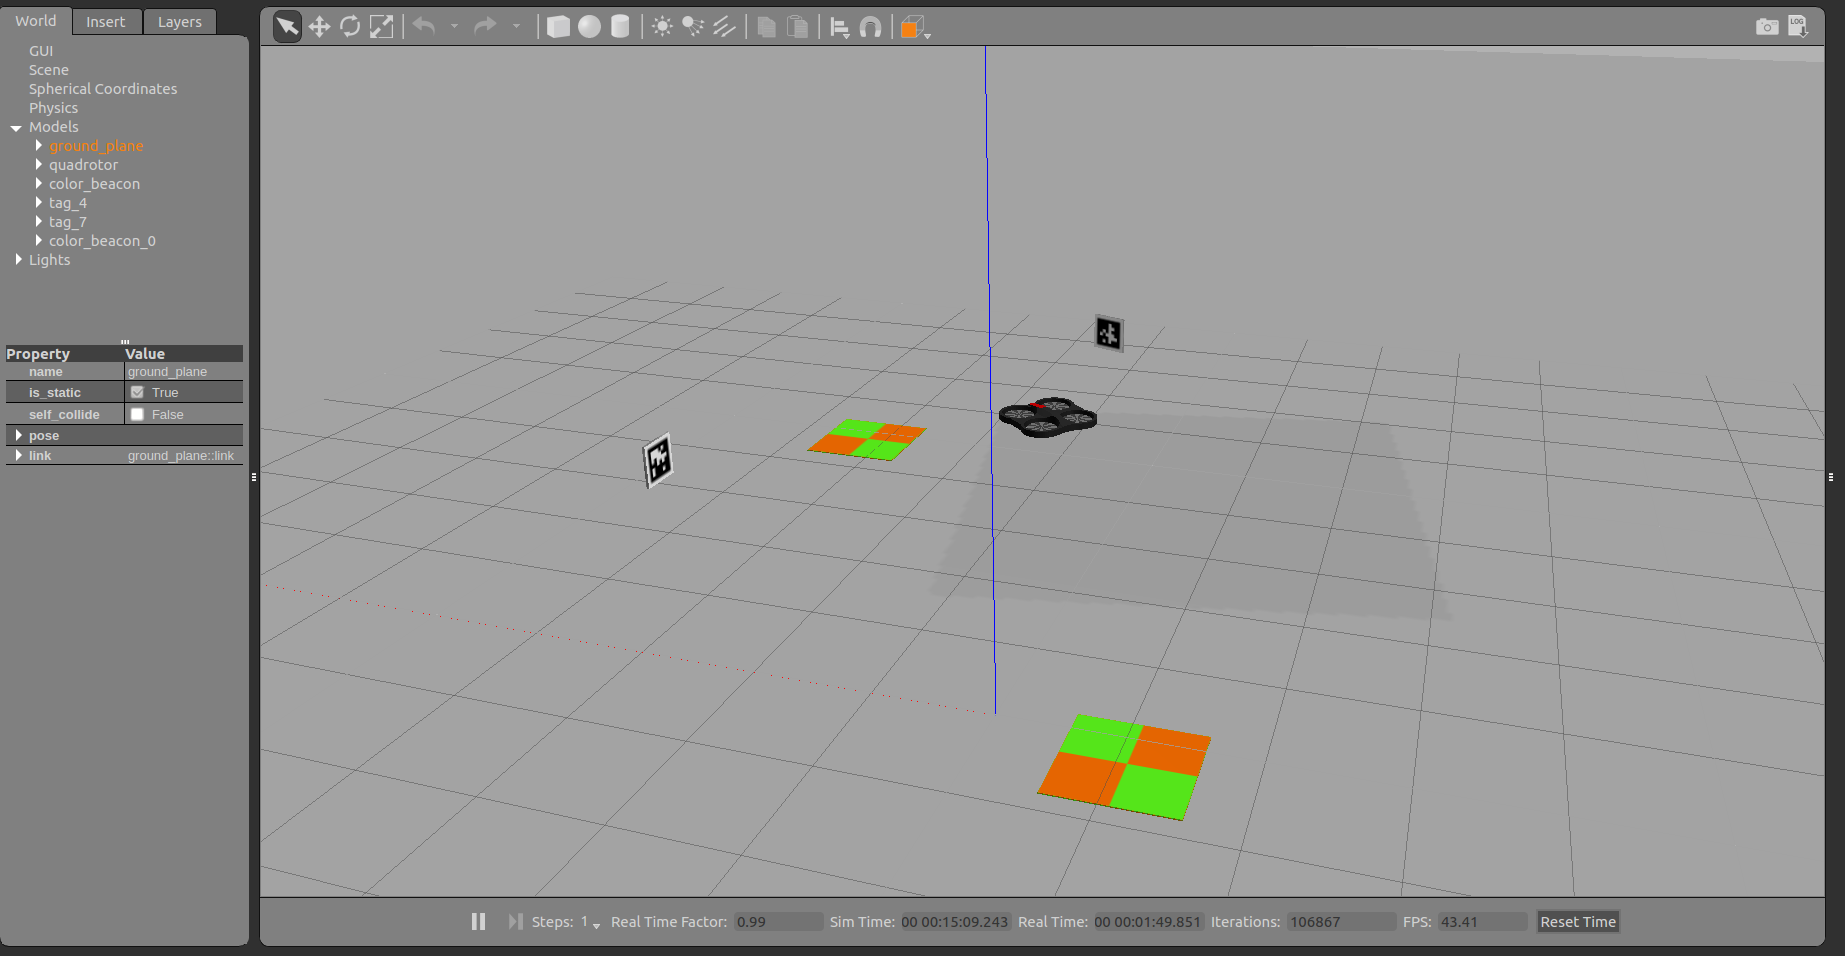
\includegraphics[width=1\textwidth]{imag/gazebo.png}
		\caption{Escenario utilizado para las pruebas unitarias en Gazebo.}
		\label{fig:Escenario Gazebo pruebas.}	
	\end{center}
\end{figure}

\subsection{Elección de balizas de despegue y aterrizaje}

Se han seleccionado las balizas de colores arlequinadas, ya que se detectó una posible limitación de las balizas AprilTags a la hora del despegue y aterrizaje. Esta limitación se debe a que si nos acercamos demasiado a las balizas, no entrarán en nuestro campo de visión y por lo tanto AprilTags dejarán de tener utilidad en esas situaciones límite \ref{fig:compararBalizasGazebo}. Con las balizas arlequinadas se puede mantener la cruceta en pantalla, siempre y cuando se mantenga la baliza en el centro de la imagen. Hay que añadir que cuanto más descendamos, más difícil será mantener la cruceta en el campo de visión.

\begin{figure}[H]
	\begin{center}
		\centering
		\subfloat[Drone simulado con baja altura] {\includegraphics[scale=0.18]{imag/simulador_balizas_cerca.png}}\hspace{10mm}
		\subfloat[Vista de la cámara vental de la baliza baliza arlequinada]{
\includegraphics[scale=0.3]{imag/baliza_arlequinada_cerca.png}}\hspace{10mm}
		\subfloat[Vista de la cámara vental de la baliza AprilTags]{
\includegraphics[scale=0.3]{imag/apriltags_cerca.png}}
		\caption{Comparación de balizas visuales en Gazebo.}
		\label{fig:compararBalizasGazebo}	
	\end{center}
\end{figure}


\subsection{Ajuste del control de navegación}

Se han realizado pruebas con las balizas de AprilTags para entender el funcionamiento y los valores devueltos. La tarea más tediosa durante esta fase ha sido la calibración de los coeficientes para el controlador PID de forma manual. Se trata de un proceso de prueba y error en el que se modifican los valores de los coeficientes, cuyo impacto sólo puede verse reflejado durante la ejecución del programa. Las observaciones en estas pruebas reflejan la facilidad con la que podemos prescindir de las componentes ID del controlador PID en un entorno virtual, ya que el ruido es prácticamente nulo y el comportamiento del drone es muy próximo al ideal.

\begin{figure}[H]
	\begin{center}
		\includegraphics[width=1\textwidth]{imag/ejecucion_completa_gazebo.png}
		\caption{Drone simulado navegando en Gazebo.}
		\label{fig:simulado_navegacion}	
	\end{center}
\end{figure}

\subsection{Ejecución típica integral}

Durante las pruebas generales se ha observado que el algoritmo es capaz de correr a una frecuencia máxima de 77 Hz por estado. Esto permite una navegación fluida y ágil, lo que se descartará cualquier fallo debido al rendimiento o velocidad de procesado de imágenes.

El despegue y aterrizaje controlado aplica dos PID, cada uno para controlar las dos dimensiones del plano paralelo a la baliza arlequinada que se encuentra en el suelo del simulador. Debido a que las imágenes de la cámara ventral y la frontal tiene el formato 4:3 y 16:9 respectivamente, los coeficientes correspondientes a la altura de la imagen serán proporcionalmente más pequeños para conseguir un control más preciso.

En el caso de la navegación autónoma en 3D \ref{fig:simulado_navegacion}, se añade complejidad aplicando un PID a una distancia objetivo predefinida, cuyos coeficientes han tenido que ser calibrados independientemente. 


Una vez termina la navegación, se activará un estado que buscará la baliza arlequinada y acto seguido iniciará el estado de aterrizaje controlado. Ha sido necesaria la calibración de la velocidad de búsqueda en espiral para que el PID del aterrizaje consiga controlar su posición encima de la baliza y evitar un bucle de búsqueda-aterrizaje continuo.

\section{Pruebas con el drone real y PC externo}

En este escenario el principal objetivo era la familiarización con el drone real y la adaptación del código a las fluctuaciones y diferencias con el simulador.

\subsection{Ajuste del control de navegación}

La primera observación fue que los coeficientes del controlador PID no aplican directamente al drone real, dotando de un comportamiento demasiado violento y nada controlado. La calibración de los coeficientes se presentaba mucho más complicada que en el simulador, por lo que para comprender mejor el funcionamiento del drone real, se modificó el componente \texttt{uav\_viewer\_py} \ref{subsec:uavviewer} para poder teleoperar con las teclas del teclado el drone. A raíz de esto se pudo comprobar el efecto de las velocidades en el drone y se modificó el código para limitar la velocidad máxima al mismo tiempo que calibrar los coeficientes en los casos en que se saturase la velocidad.

\subsection{Desfase entre imágenes y órdenes}

Durante las pruebas se pudo observar un desfase entre las órdenes y las imágenes (provocado por \texttt{slam\_markers} \ref{subsec:slam Markers}). 

Se pudo dar solución a al desfase sustituyendo slam\_markers por un módulo integrado la parte de percepción del estado de navegación. Se caracterizó la diferencia entre el rendimiento de la nueva aplicación, ejecutando a una media de 33 Hz por ciclo a diferencia de slam\_markers, cuyo rendimiento oscilaba entre los 3 y 4 Hz (insuficientes para realizar el control). 

\subsection{Problemas con la detección de las balizas arlequinadas}

Una tarea que retrasaba la ejecución de los experimentos estaba provocada por el efecto que tenía la variación de luz en la calibración de las balizas arlequinadas.La variación de luz fue mitigada desarrollando la herramienta CalibrationTool \ref{sec:calibrationtool}. Estas dos soluciones permitieron realizar con éxito las pruebas unitarias que fueron grabadas como prueba.
\begin{figure}[H]
	\begin{center}
		\centering
		\subfloat[] {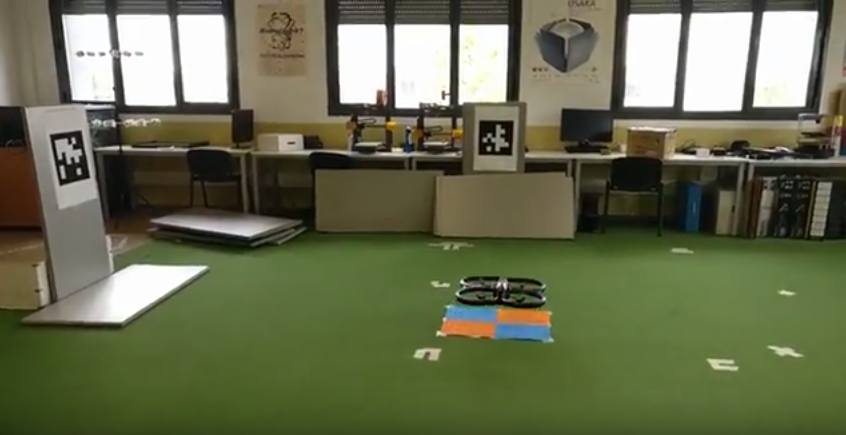
\includegraphics[scale=0.35]{imag/despegue1.png}}\hspace{5mm}
		\subfloat[] {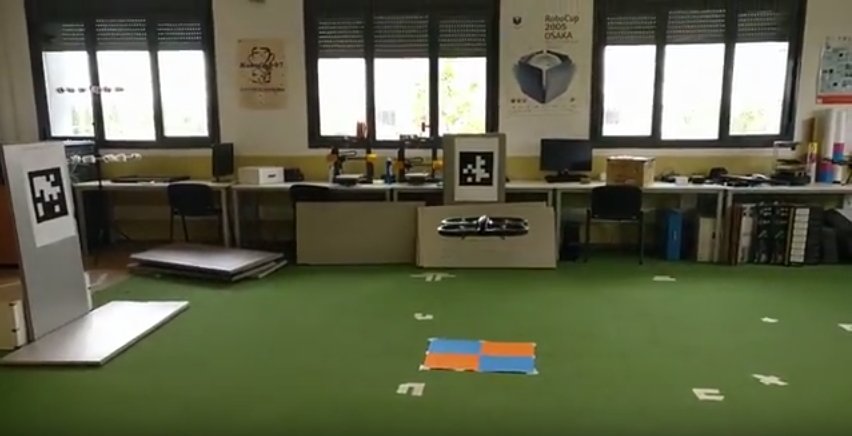
\includegraphics[scale=0.35]{imag/despegue2.png}}\hspace{5mm}
		\label{fig:despegueReal}	
	\end{center}
\end{figure}

\begin{figure}[H]
	\begin{center}
		\centering
		\subfloat[] {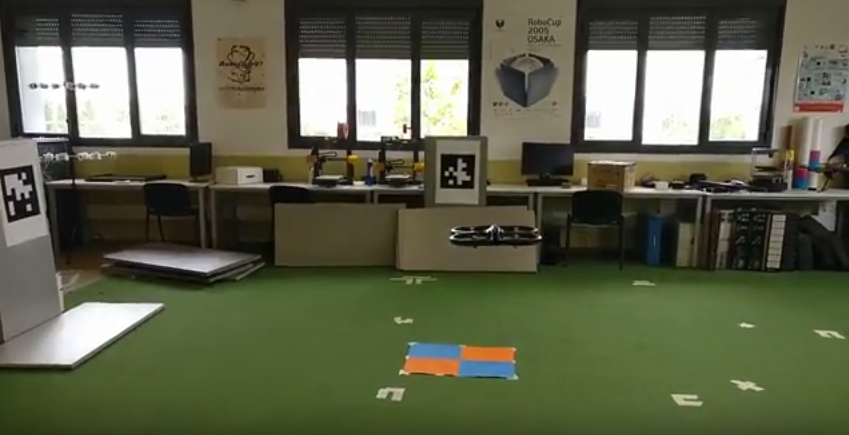
\includegraphics[scale=0.35]{imag/despegue3.png}}
		\caption{Secuencia de despegue.}
		\label{fig:despegueReal2}	
	\end{center}
\end{figure}
\subsection{Ejecución típica integral}

Se ha conseguido realizar de forma satisfactoria diferentes ejecuciones en las que se logrado despegar y aterrizar de forma controlada en una única baliza arlequinada y navegar a las cuatro balizas de AprilTags que se han desplegado a lo largo del laboratorio \ref{fig:balizasDesplegadas2}.

\begin{figure}[H]
	\begin{center}
		\centering
		\subfloat[Baliza arlequinada] {\includegraphics[scale=0.8]{imag/baliza_color.png}}\hspace{5mm}
		\subfloat[Baliza AprilTags 4] {\includegraphics[scale=0.8]{imag/baliza_april1.png}}
	\end{center}
\end{figure}

\begin{figure}[H]
	\begin{center}
		\centering
		\subfloat[Baliza AprilTags 7] {\includegraphics[scale=0.8]{imag/baliza_april2.png}}\hspace{5mm}
		\subfloat[Baliza AprilTags 16] {\includegraphics[scale=0.8]{imag/baliza_april3.png}}\hspace{5mm}
		\subfloat[Baliza AprilTags 30] {\includegraphics[scale=0.8]{imag/baliza_april4.png}}
		\caption{Balizas desplegadas en el laboratorio.}
		\label{fig:balizasDesplegadas2}	
	\end{center}
\end{figure}

Se encontraron problemas menores relacionados con la deriva del robot, en concreto durante el estado de búsqueda rotacional, en la que el movimiento que describe es realmente un toroide, desplazándose continuamente mientras gira. El aumento de la velocidad rotacional disminuyó el problema, pudiendo grabar un vídeo como validación de la prueba.

\begin{figure}[H]
	\begin{center}
		\centering
		\subfloat[] {\includegraphics[scale=0.4]{imag/navegacion1.png}}\hspace{5mm}
		\subfloat[] {\includegraphics[scale=0.4]{imag/navegacion2.png}}\hspace{5mm}
		\label{fig:navegacionReal1}	
	\end{center}
\end{figure}

\begin{figure}[H]
	\begin{center}
		\centering
		\subfloat[] {\includegraphics[scale=0.4]{imag/navegacion3.png}}\hspace{5mm}
		\subfloat[] {\includegraphics[scale=0.4]{imag/navegacion4.png}}
		\caption{Secuencia de navegacion.}
		\label{fig:navegacionReal2}	
	\end{center}
\end{figure}

En comparación a la ejecución del simulador, la frecuencia máxima a la que se ha podido ejecutar la aplicación ha sido 33 fotogramas por segundo. Este descenso se debe principalmente a que la resolución de las imágenes del simulación son mucho más pequeñas comparadas con las del drone real (640x480 píxeles para el simulador y 1280x720 píxeles para el drone real).

\section{Pruebas con el drone real y un miniordenador}

En este escenario el principal objetivo era comprobar los límites físicos del drone real y probar la posibilidad de crear un sistema totalmente autónomo con el Intel Stick Compute a bordo. 

\subsection{Preparación y configuración del miniordenador}

Se ha instalado la versión de Ubuntu 16.04 para ser compatible con los requisitos anteriormente citados. Es necesario añadir que se ha instalado JdeRobot en su versión más reciente y que se ha configurado un servidor SSH para realizar las comunicaciones con el dispositivo cuando esté operando y no esté conectado el HDMI a un monitor externo. Este dispositivo irá acoplado mediante cinta adhesiva.

\begin{figure}[H]
	\begin{center}
		\includegraphics[width=1\textwidth]{imag/ics_drone_calibrated.jpg}
		\caption{Intel Compute Stick acoplado en Ar.Drone 2.}
		\label{fig:intelAcoplado}	
	\end{center}
\end{figure}

Además de haber instalado Ubuntu en la versión 16.04, junto a todas las dependencias y bibliotecas necesarias para correr la aplicación, se ha configurado el asistente de la red Wi-Fi para que se conecte de manera automática cuando detecte que la red que genera el drone. Se configuró la IP como estática para poder acceder de forma remota y conocer la dirección exacta de nuestra unidad de computación externa. 

Por último, se ha configurado un servidor utilizando la tecnología OpenSSH de manera que se inicie durante el lanzamientos del Sistema Operativo y que escuche en el puerto 22998. Esto  aportará una capa de seguridad, actualmente no existente además de habilitar el acceso remoto.

\subsection{Teleoperación con miniordenador a bordo}

El primer paso sería realizar una prueba teleoperando la infraestructura \ref{fig:intelAcoplado} desde nuestra herramienta uav\_viewer\_py modificado para observar cualquier cambio en el comportamiento. Lamentablemente el drone se volvía completamente inestable: desde el despegue, pasando por movimientos erráticos y no controlados, independientemente del envío de órdenes o no al drone. La limitación de potencia por parte del drone es la culpable, por lo que la única solución posible es la de realizar las pruebas sin montar a bordo el co-procesador.

\subsection{Retardo detectado en uav\_viewer\_py}

La ejecución de las pruebas unitarias reflejaba un comportamiento muy oscilante debido posiblemente a algún tipo de retardo, por lo que las primeras sospechas apuntaban a la diferencia de rendimiento entre el Intel Compute Stick y el ordenador externo de la sección anterior. Se caracterizó este retardo, mostrando valores de hasta más de un segundo en algunas de las iteraciones de los estados. Para descartar posibles problemas de rendimiento, se analizó el periodo de ejecución del estado, el consumo de recursos como el procesador, la memoria RAM y el ancho de banda utilizado. Sin embargo, los resultados de estas pruebas mostraban una frecuencia mínima de 20 Hz por ejecución, chocando con los valores previamente obtenidos.

Una investigación mas profunda llevó a la conclusión de que la herramienta \texttt{uav\_viewer\_py} que se utilizó para obtener las imágenes del drone en remoto, provocaba una saturación en el canal Wi-Fi, por lo que la solución se basó en la omisión de esta aplicación durante las pruebas con el Intel Compute Stick.



\subsection{Ejecución típica con el miniordenador en tierra}

Para iniciar la aplicación, necesitaremos acceder remotamente mediante el siguiente comando: 

\begin{lstlisting}[backgroundcolor=\color{gray!15}]
ssh 192.168.1.3 -p 22988
\end{lstlisting}

Una vez dentro, lanzaremos la aplicación de manera que la ejecución se realice en el \textit{Intel Compute Stick}.

Para prevenir cualquier accidente, se ha desarrollado un programa muy sencillo, cuya única misión es la de enviar la señal de aterrizaje al drone. Este comando evita la ejecución de futuras órdenes y asegura que el aterrizaje se realizará en el menor tiempo posible.

Se pudieron ejecutar sin problemas las pruebas unitarias, dando paso a la realización de la última prueba global o ensayo general. Este fue gratamente satisfactorio, a pesar de presentar un comportamiento ligeramente inferior en cuanto a precisión y agilidad comparado con las pruebas de la fase anterior, oscilando en mayor medida.

%\lhead[]{CAPÍTULO \thechapter. Conclusiones}
\chapter{Conclusiones}\label{cap.conclusiones}

En este capítulo analizaremos si los objetivos \ref{sec:objetivos} planteados se han cumplido y se recapitulan las soluciones desarrolladas y los resultados obtenidos. Adicionalmente, sugeriremos las posibles líneas futuras de investigación por las que se puede extender este TFG. En líneas generales el objetivo global se ha alcanzado satisfactoriamente. Se ha conseguido por primera vez en el proyecto JdeRobot la navegación completamente autónoma en un entorno 3D utilizando un drone real, además de abrir la puerta al uso de miniordenadores embarcados a bordo de drones que tengan motores más potentes que los del Ar.Drone 2 de Parrot.

\section{Conclusiones}

Gran parte del trabajo aquí expuesto no ha formado parte de la programación directamente, sino que incluye el tiempo de investigación, aprendizaje de herramientas, tecnologías y habilidades que han tenido que ser adquiridas o adaptadas para programar con éxito la solución. Otra parte que se encuentra oculta detrás de los programas es el mérito de haber realizado los experimentos en un drone real cuyo comportamiento es inestable, en el que el ruido de los sensores condiciona el resultado de las pruebas y en el que la duración de las baterías reduce el número de pruebas diarias que se pueden realizar.

A continuación analizamos todos los subobjetivos para extraer las conclusiones que hemos obtenido en cada uno de ellos, recapitulando a la vez cómo han sido conseguidos:

\begin{enumerate}
	\item \textit{Integración del módulo de autolocalización 3D a partir de balizas visuales:} El funcionamiento ha sido validado mediante pruebas unitarias. Se ha reimplementado en Python el algoritmo que utilizaba \texttt{slam\_markers} y se ha integrado dentro del nodo \texttt{3DPathFollower}. Este módulo es capaz de estimar las coordenadas relativas con respecto a una baliza visual correctamente, permitiendo a la aplicación final realizar las correcciones necesarias en tiempo real y con la precisión necesaria.
	\item \textit{Desarrollo e integración de un módulo de navegación por balizas visuales:} Se ha desarrollado e integrado un PID capaz de ser aplicado para las diferentes balizas visuales utilizadas, aprovechando los recursos y mejorando el rendimiento de nuestra aplicación. Además, se ha ajustado el control del pilotaje tanto para escenarios simulados como para el drone real.
	\item \textit{Programación del comportamiento del drone en un autómata de estados finito:} Se han integrado la autolocalización, los controladores de aterrizaje, de despegue y de navegación siguiendo balizas visuales en un único autómata compacto, basado en 8 estados conectados a través de transiciones. Esto ha sido posible con la ayuda de \textsc{Visual States}.
	\item \textit{Validación experimental en el cuadricóptero  real:} Se han realizado pruebas tanto en el cuadricóptero simulado en Gazebo como principalmente con el cuadricóptero real Ar.Drone 2 de Parrot. Estas pruebas han sido tanto unitarias como globales, mostrando las capacidades de la navegación autónoma en 3D utilizando por primera vez balizas visuales. El comportamiento es ágil y preciso, además de eficiente ya que el algoritmo es capaz de ejecutar a una frecuencia de 33 Hz. 
	
	Los resultados obtenidos con miniordenador a bordo se han visto limitados debido a las restricciones de potencia del drone, que imposibilitan una prueba completamente a bordo. Aun así, se ha conseguido validar experimentalmente las capacidades de procesamiento del Intel Compute Stick \ref{sec:ics} de forma externa, dando como resultado un comportamiento ágil, suficientemente preciso, y con una frecuencia de ejecución de 20Hz, no muy diferente de la de un computador. De esta manera se deja abierta la puerta a posibles futuras aplicaciones con comportamientos autónomos totalmente a bordo. Se ha validado experimentalmente a través de la prueba global, en la que se ha ejecutado de principio a fin el algoritmo sin intervención externa de un humano, completando todos los estados y finalizando el ejercicio con el aterrizaje y detención del drone en la posición designada.
	
	
	%\item{\textbf{Diseño y desarrollo de una aplicación para la calibración de balizas bicolor arlequinadas:} Se ha conseguido desarrollar una aplicación que a través de una interfaz gráfica, modifique en tiempo real los filtros de color y que genere como resultado un fichero de configuración xml, el cual ha probado su utilidad ya que ha facilitado su futura utilización frente a cambios de luz o diferentes combinaciones de colores.}
	%\item{\textbf{Reimplementación y desarrollo de módulos de búsqueda:} Se ha conseguido desarrollar los dos módulos propuestos: uno dedicado para las balizas arlequinadas y otro para las balizas AprilTags. Ambos han sido validados experimentalmente y juntos han aumentado la autonomía a la hora de navegar del drone.}
	%\item{\textbf{Desarrollo de la inteligencia del dron materializándola en un autómata de estados finito:}	La aplicación 3DPathFollower es el resultado de este desarrollo e integración, junto con la ayuda de \textsc{Visual States}. Los estados han facilitado la realización de pruebas experimentales unitarias y globales. El algoritmo ha sido satisfactoriamente probado de principio a fin en un drone real y utilizando el co-procesador como unidad de procesamiento. Los estados creados dotarán de una base para futuras investigaciones y un ejemplo para generar otros algoritmos y aprovechar la modularidad que ofrece \textsc{Visual States}.}
	%\item{\textbf{Configuración del co-procesador a bordo del dron:} Este objetivo se ha visto modificado debido a las restricciones del dron, dado que no tenía suficiente potencia para ejecutar el comportamiento enviado por el co-procesador. Aun así, se ha conseguido configurar satisfactoriamente la infraestructura necesaria para externalizar el procesamiento en el Intel Compute Stick \ref{sec:ics}, además de aportar las herramientas y configuración necesarias para la ejecución y detención en remoto.}
	%\item{\textbf{Validación experimental en el cuadricóptero real:} Se han realizado satisfactoriamente tanto pruebas unitarias como globales, demostrando la efectividad de la prueba de concepto a la hora de utilizar una unidad como co-procesador y se ha mostrado la navegación autónoma en 3D utilizando por primera vez balizas de tipo AprilTags. La comparativa entre la ejecución tradicional y la nueva ha sido positiva, a pesar de que los resultados no son totalmente favorables para el co-procesador, el comportamiento y el rendimiento están muy cerca y no han supuesto un problema real para la ejecución de las pruebas. Esto abre la puerta a futuras nuevas aplicaciones utilizando esta infraestructura y cambiando posiblemente el dron por otro más potente u otro formato (como por ejemplo un avión).}
\end{enumerate}

Se ha aportado una nueva herramienta a la plataforma de JdeRobot, que ahora cuenta con un ejemplo de probado en un drone real navegación de forma autónoma, desde el despegue hasta el aterrizaje, realizando desplazamientos controlados. 

Todo el material audiovisual y avances que han ido teniendo lugar se pueden consultar en la Wiki oficial del proyecto: \url{http://jderobot.org/Andresjhe-tfg}

El código está subido al repositorio oficial del TFG y puede ser accedido sin restricciones para su revisión y mejora: \url{https://github.com/RoboticsURJC-students/2014-tfg-Andres-Hernandez/}

\section{Trabajos futuros}
Con este proyecto se han abierto algunas fronteras inexploradas lo que facilita el desarrollo de nuevas aplicaciones o la mejora de las ya existentes, en concreto en el ámbito de la navegación autónoma y la utilización de un miniordenador a bordo. A continuación se proponen algunas posibles líneas futuras a partir de los resultados y la experiencia obtenida durante la realización de este TFG:

\begin{itemize}
	\item Aumentar la complejidad de la navegación o probar en un escenario de exteriores. Ambas vías están directamente relacionadas con la mejora de los algoritmos desarrollados. 
	\item Sustitución de los algoritmos de visión por otros más sofisticados como técnicas de SLAM para autolocalización o el uso de \textit{DeepLearning}. Aumentaría la robustez y la cantidad de escenarios en los que puede ser utilizados, a pesar de que se sacrificaría eficiencia computacional y  en latencia.
	\item Sustitución del drone existente. La mayor dificultad a la hora de cumplir todos los objetivos ha estado directamente relacionada con las limitaciones del drone actual (derivas, falta de empuje vertical, ruido o defectos en sensores, etcétera). Un nuevo drone más potente puede ser la solución a los problemas encontrados.
\end{itemize}

\addcontentsline{toc}{chapter}{Bibliografía}
\begin{thebibliography}{X}
\bibitem{AlbertoMartin} \textsc{Alberto Martín Florido.} Navegación visual en un cuadricóptero para el seguimiento de objetos. \textit{Trabajo Fin de Grado}, URJC, 2014.	

\bibitem{DanielYague} \textsc{Daniel Yagüe Sánchez.} Cuadricóptero AR.Drone en Gazebo y JdeRobot. \textit{Proyecto Fin de Carrera,} URJC, 2014.

\bibitem{AlbertoLopez} \textsc{Alberto López-Cerón Pinilla.} Autolocalización visual robusta basada en marcadores. \textit{Trabajo Fin de Master}, URJC, 2015.

\bibitem{ManuelZafra} \textsc{Manuel Zafra Villar.} Seguimiento de rutas 3D por un drone con autolocalización visual con balizas. \textit{Trabajo Fin de Grado} URJC, 2016.

\bibitem{JorgeVela} \textsc{Jorge Vela Peña.} Despegue, navegación y aterrizaje visuales de un drone usando JdeRobot. \textit{Trabajo Fin de Grado} URJC, 2017. 

\bibitem{JesusSaiz} \textsc{Jesús Saiz Colomina.} Programación de un dron para seguimiento autónomo de trayectorias en 3D. \textit{Trabajo Fin de Grado} URJC, 2018.

%\bibitem{AprilTags2} \textsc{John Wang} y \textsc{Edwin Olson}, AprilTag 2: Efficient and robust fiducial detection. \textit{Proceedings of the IEEE/RSJ International Conference on Intelligent Robots and Systems (IROS)}, Octubre 2016.

%\bibitem{WorldRobotics} \textsc{International Federation of Robotics}, World Robotics 2017

\end{thebibliography} 

\end{document}
